Due to the immense computational requirements of this analysis and that of \parencite{Lee2022MeasurementDetector}, efforts were directed in parallel to investigating enhancing the simulation pipeline with statistical methods. In particular, normalizing flows were examined as a way to reduce computational needs for correction factor determinations, as well as for assisting in solving inverse problems. 

    \textcolor{red}{ The event generation described earlier in this chapter can be posed as generating a 16xn truth-level dataset, where n is the number of DV$\pi^0$P events produced, with each event containing four 4-vectors to yield 16 elements of information. This information must be transformed in a realistic way into the four-momenta typically observed after event reconstruction, data processing, and exclusivity cuts are applied. Traditionally this is achieved through the simulation processing described in previous sections, involving swimming each particle through microphysics simulations and applying reconstruction algorithims to the resulting simulated detector hits. }
    

    \textcolor{red}{  Thus, we stand to save a huge amount of processing time if we can train a model on the distribution generated by only several million microphysics generated datapoints, and sample the rest from the trained model. Several groups in particle physics are trying to develop similar methods, for example, training flows to reduce LHC simulation time \parencite{Weisser2021ThePhysics} or work at MIT's IAIFI focused on speeding up aspects of Lattice QCD by a factor of up to 1,000 \parencite{Kanwar2020EquivariantTheory}.}
    
\subsection{Inverse Transforms and Autoregressive Flows}
    
    
    Normalizing flow are effective models to learn a probability distribution $p(x)$ when a sample data set $X=\{x\}$ following the distribution is given. The basic idea is a series of transformation $g_i$'s, which are referred to as flows, transforms a prior probability $p(z)$ distributions into the target distribution $p(x)$. That is
    \begin{align}
        \mathbf{x} =& g_N \circ g_{N-1}\circ ... \circ g_1 (\mathbf{z}), \\
        \mathbf{z} =& f_1 \circ ... \circ f_{N-1} \circ f_N (\mathbf{x}), \label{eqn:invertible}
    \end{align}
    where $f_{N-i+1}\equiv g_i^{-1}$ following \parencite{Kobyzev2021NormalizingMethods}'s convention. Both $\mathbf{x}$ and $\mathbf{z}$ are vectors of the same dimension $d$. From the eq.~\ref{eqn:invertible}, $g_i$ requires an invertibility condition. An intermediate flow $\mathbf{z_i}$ is defined as follows.
    \begin{align}
    \mathbf{z_i} =&g_i \circ ... \circ g_1(\mathbf{z}), \label{eqn:forward}\\
        =&f_{i+1}\circ ...f_N(\mathbf{x}), \label{eqn:backward}
    \end{align}
    where the flow is expressed in forward direction at eq.~\ref{eqn:forward}, and in backward direction at eq.~\ref{eqn:backward}. Therefore, $\mathbf{z_{i+1}}=g_i (\mathbf{z_i})$ and $\mathbf{z_i} = f_{N-i+1}(\mathbf{z_{i+1}})$ for one flow, or layer. If the $f_i$'s are differentiable, the PDF evolves as follows.
    \begin{align}
     p(\mathbf{z_{i+1}})=& p(\mathbf{z_i})|\frac{\partial f_{N-i+1}}{\partial \mathbf{z_i}}| =p(\mathbf{z_i})|\frac{\partial g_{i}^{-1}}{\partial \mathbf{z_i}}|\\
     \log p(\mathbf{z_{i+1}}) =& \log p(\mathbf{z_i}) + \log|\frac{\partial g_i^{-1}}{\partial \mathbf{z_i}}| \label{eqn:logprob}\\
     \log p(\mathbf{x}) =& \log p(\mathbf{z}) + \sum\limits_{i=1}^N \log|\frac{\partial g_i^{-1}}{\partial \mathbf{z_i}}|.
    \end{align}
    Eq.~\ref{eqn:logprob} is useful to define the forward and the backward propagation of each layer.
    Once the NF model is trained to learn the distribution $g: p(z)\rightarrow p(x)$, it is possible to sample $x$ using sampled $z$. \parencite{Gao2020EventFlows} showed that the Nonlinear Independent Component Estimation (NICE) \parencite{Dinh2014NICE:Estimation} implementation of NF performs well by comparing the technique to existing methods in terms of efficiencies that are defined as average weight during the generation.

\subsection{Exploration of Simulation Speedup with UNMAF}

    Motivated by \parencite{Weisser2021ThePhysics}'s work, Masked Autoregressive Flows were used for this investigation (MAF, \cite{Papamakarios2017MaskedEstimation}), which is one of the generalized versions of NICE. The MAF starts from a simple fact that $p(z_{i}) = \prod\limits_{j}p(z_{i,j}|\mathbf{z}_{i,0:j-1})$. The component $z_{i,j}$ is the $j$-th component of $z_i$, and the vector $\mathbf{z}_{i,0:j-1}$ is defined as $\{z_{i, 0}, ..., z_{i, j-1}\}$. The transformation is finally defined as
    \begin{align}
        z_{i+1, j}=& \sigma_{i, j} z_{i, j} + \mu_{i+1, j}.
    \end{align}
    The moments $\mu_{i+1, j}$ and $\sigma_{i, j}$ are the mean and standard deviation of $p(z_{i+1,j}|\mathbf{z}_{i+1,0:j-1})$ ($\equiv p(z_{i+1,0})$ for $j=0$). We train the flows to learn $\mu_{i+1, j}$'s and $\sigma_{i, j}$'s, and sample $p(\mathbf{x})$. 

    More specifically, Unconstrained Monotonic Neural Networks (UMNN, \cite{Wehenkel2019UnconstrainedNetworks}) MAF architecture was utilized, as it is able to learn noncontinuous distributions from stacked data files. \parencite{Wehenkel2019UnconstrainedNetworks} demonstrates that the UMNN-MAF successfully learn discontinuous distributions, and that sampling is possible even in the case that the transformation is not analytically invertible.
    
    A training set of 5M data points was generated and processed using the traditional simulation tools discussed earlier in this chapter. This yielded a training input vector $\mathbf{x}$ with dimensions of $5\text{M}\times16$, where each element is just a floating point number.

    \subsubsection*{Architecture and Training}
        Our architecture consists of 16 layers of UMNN-MAF with 32 hidden variables per layer in the 16-feature case, and consisted of 6 layers with 80 hidden variables per layer in the 4-feature case. After many trials of different combinations of hyper parameters and flow models, we found that an effective training method to use 10000 epochs with each iteration using randomly sampled training data sets of 400$\times$16 dimension from the initial 5M data points generated by physics simulations. To evaluate our model, we sampled 100k data points, $\mathbf{x_1}$, from the physics simulation set which were not included in training, and generated 100k data points, $\mathbf{x_2}$, using our trained model.The Earth Mover's Distance (EMD), calculable as the Wasserstein-1 Distance \parencite{Dobrushin1970PrescribingDistributions} was evaluate between $\mathbf{x_1}$ and $\mathbf{x_2}$. Since our sample data size was somewhat small, we sampled a second set of 100k data points, $\mathbf{x_1'}$, from the physics simulation set, and calculated EMD values between  $\mathbf{x_1}$ and $\mathbf{x_1'}$, to have a benchmark to compare with the metrics from the normalized flow comparison.
        
        
    
        Training the NF models was relatively fast, for the 16-feature model taking about 1 hour on a GPU (NVIDIA Quadro RTX 5000) or about 10 hours on a CPU (Intel Xeon E-2276M). On the other hand, sampling from the trained model was considerably slower; the 16-feature trained NF model generated datapoints at a rate of about 4 Hz, which is only a factor of 10 times faster than the traditional method of simulating the processes' microphysics. 
        
        \parencite{Wehenkel2019UnconstrainedNetworks} and \parencite{Papamakarios2017MaskedEstimation} explains this behavior as follows. The Masked Autoencoder for Distribution Estimation (MADE, \parencite{Germain2015MADE:Estimation}), which is a building block of MAF allows the training to be done in parallel using GPUs. Sampling data points from the trained MAF takes significant amount of time because the model requires $\mathbf{z}_{i,0:j-1}$ to sample $\mathbf{z}_{i,j}$. There is a computational trade-off in Inverse Autoregressive Flow (IAF, \parencite{Kingma2016ImprovingFlow}, which trains the model slowly but samples fast. T

    To improve training, use a quantile transformation on all features in preprocessing. 
    %I.e. "from sklearn.preprocessing import QuantileTransformer"
    
    \begin{figure}[H]
        \centering
        \begin{minipage}{.3\textwidth}
        
            \centering
           % Electron
            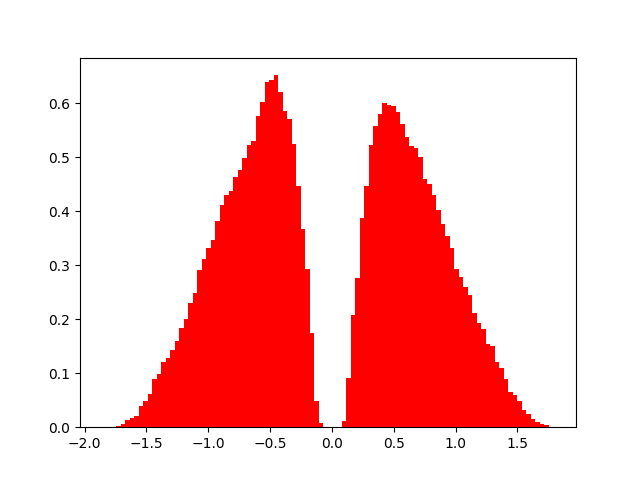
\includegraphics[width=.99\textwidth,trim={3cm 0 0 0},clip]{Chapters/Ch3-Simulations/normalizing_flows/pics/MeetingFigures/Bobby/QT/feature0_noQT.png}
            %\caption[Placeholder Short text]{(a)}
            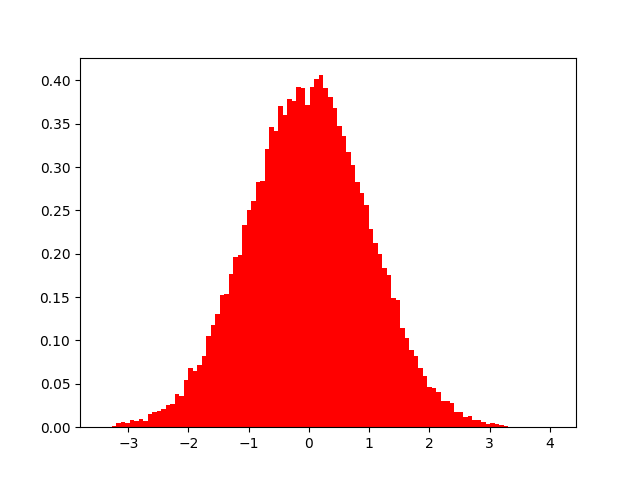
\includegraphics[width=.99\textwidth,trim={3cm 0 0 0},clip]{Chapters/Ch3-Simulations/normalizing_flows/pics/MeetingFigures/Bobby/QT/feature0.png}
    
            %\caption[Placeholder Short text]{(c)}
        \end{minipage}%
        \begin{minipage}{.3\textwidth}
        
            \centering
           % Electron
            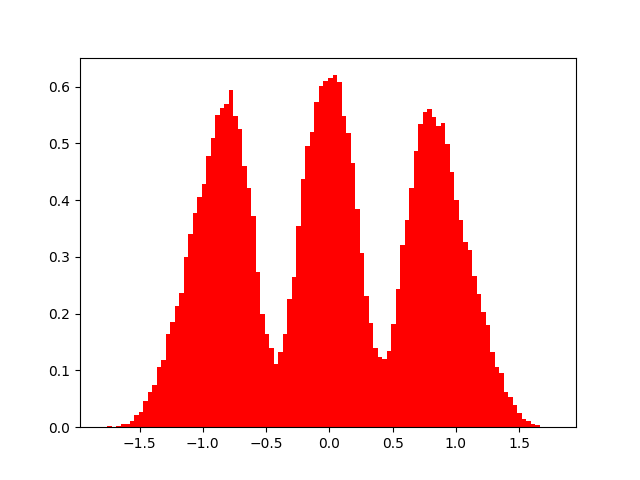
\includegraphics[width=.99\textwidth,trim={3cm 0 0 0},clip]{Chapters/Ch3-Simulations/normalizing_flows/pics/MeetingFigures/Bobby/QT/feature1_noQT.png}
            %\caption[Placeholder Short text]{(a)}
            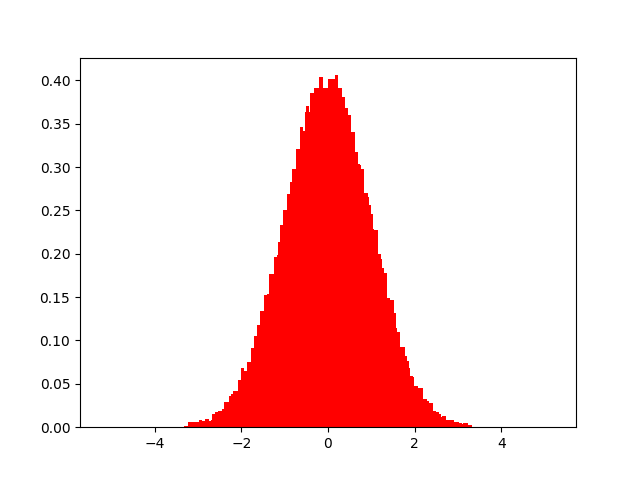
\includegraphics[width=.99\textwidth,trim={3cm 0 0 0},clip]{Chapters/Ch3-Simulations/normalizing_flows/pics/MeetingFigures/Bobby/QT/feature1.png}
    
            %\caption[Placeholder Short text]{(c)}
        \end{minipage}%
        \begin{minipage}{.3\textwidth}
        
            \centering
           % Electron
            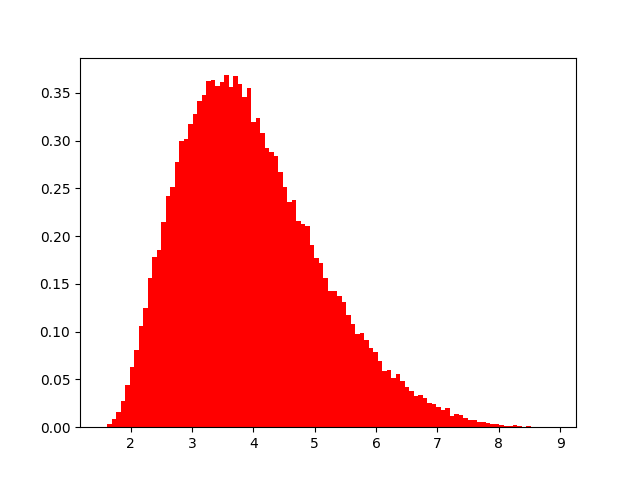
\includegraphics[width=.99\textwidth,trim={3cm 0 0 0},clip]{Chapters/Ch3-Simulations/normalizing_flows/pics/MeetingFigures/Bobby/QT/feature2_noQT.png}
            %\caption[Placeholder Short text]{(a)}
            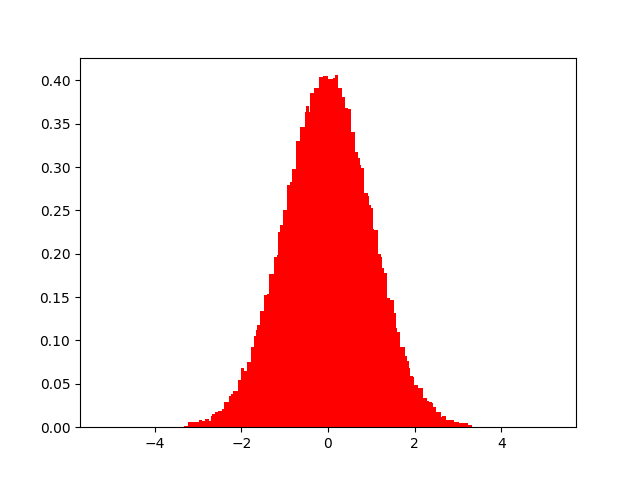
\includegraphics[width=.99\textwidth,trim={3cm 0 0 0},clip]{Chapters/Ch3-Simulations/normalizing_flows/pics/MeetingFigures/Bobby/QT/feature2.png}
    
            %\caption[Placeholder Short text]{(c)}
        \end{minipage}%
        \caption[Placeholder Short text]{Feature distributions before (top) and after (bottom) quantile transforms}
        \label{fig:16features5}
    \end{figure}

        
        Quantile transformations, also known as quantile-quantile (QQ) mapping, play a vital role in statistical analysis. Essentially, the method involves transforming the data to follow a uniform distribution, which is then inverted to follow any other specified distribution. Formally, given a random variable $X$ and its cumulative distribution function $F$, the transformed variable $X^*$ is defined as $X^* = F^{-1}(F(X))$, where $F^{-1}$ is the quantile function of the target distribution. The power of quantile transformations lies in their ability to transform data to follow any desired shape, which makes them especially useful in areas such as machine learning, where they are used for data normalization and generative modeling.

        \begin{figure}[H]
        \centering
        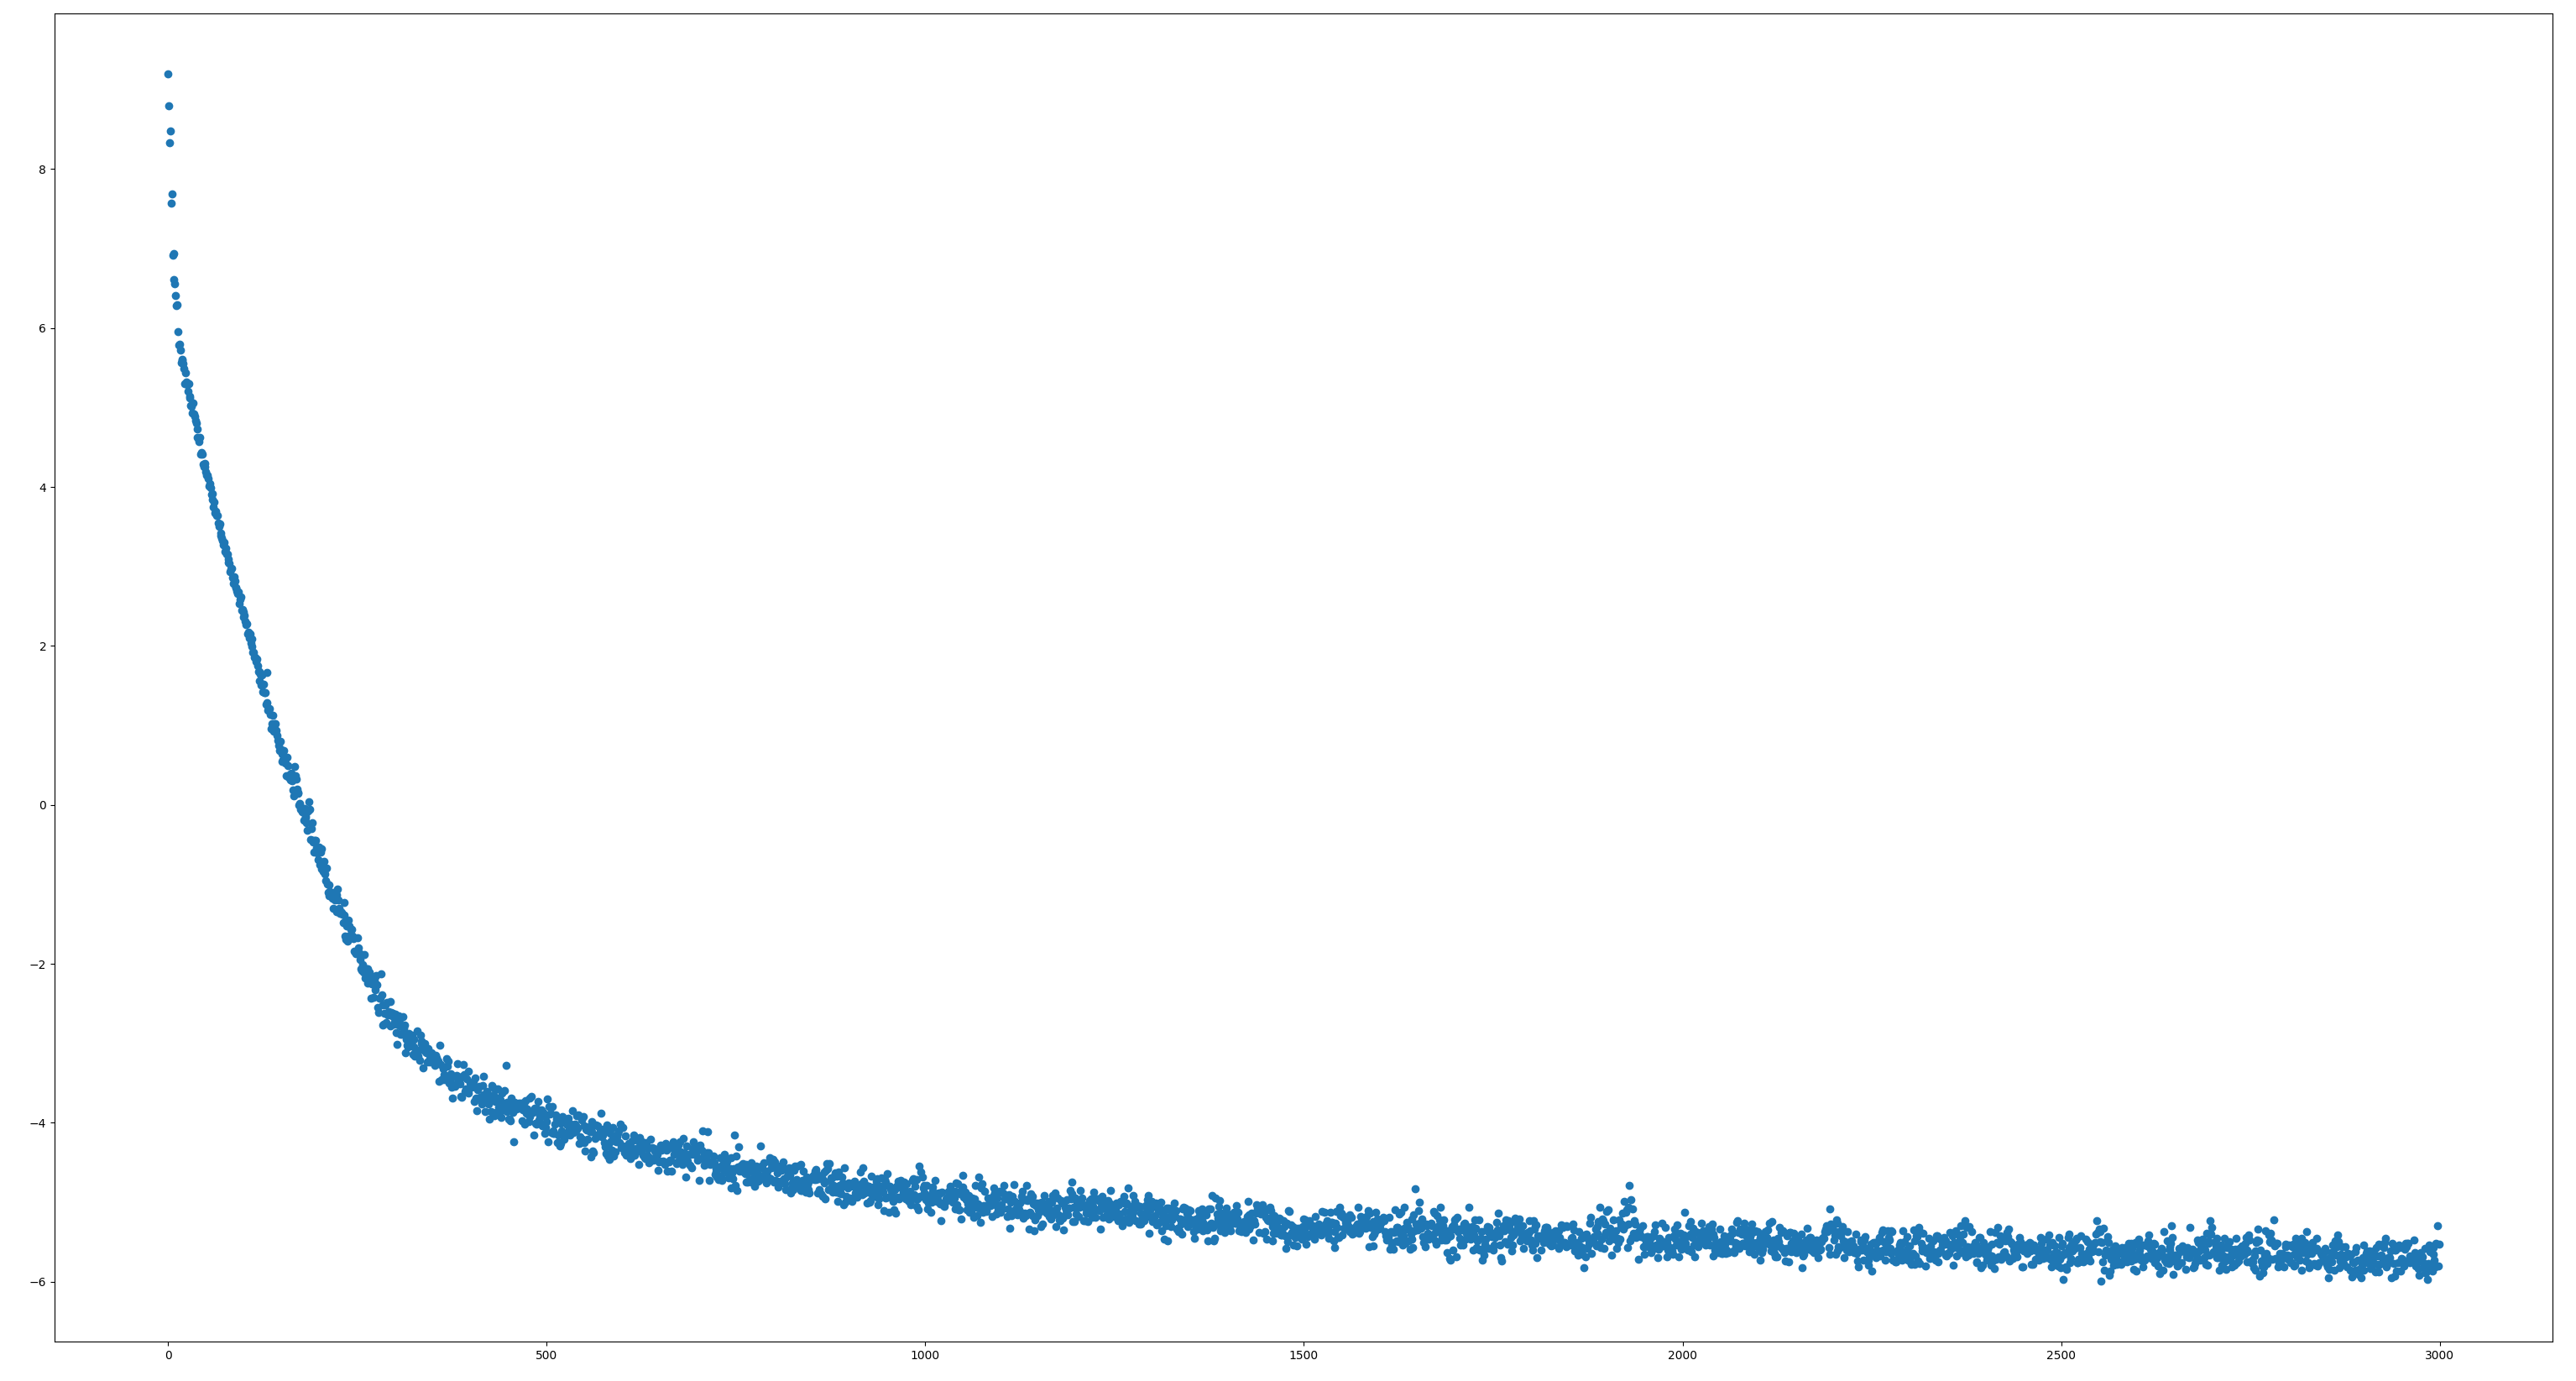
\includegraphics[width = 0.5\textwidth]{Chapters/Ch3-Simulations/normalizing_flows/pics/MeetingFigures/Bobby/LearningRate/learning_rate_25e-5_with_QT.png}
        \label{fig: jul8_pion_comparison4}
        \caption[Placeholder Short text]{Epoch (horizontal) vs Training Loss (vertical). Training loss vs. epoch with LR=2.5e-4, using Quantile Transforms }
        \end{figure}



    \subsubsection{Forward Results from Trained Model}
        Figure \ref{fig:16features} shows the feature distributions of samples from this trained model, with each plot also showing the Earth Mover's Distance between the NF model data, and sample data from the microphysics distribution.
    
        
        In general, the 16-feature trained NF model produces similar results to the traditional simulation's distribution, but fine details were difficult to reproduce. In particular, hard distribution cutoffs that exist in the traditional distribution due to the enforcement of conservation laws and the physics detector edges were not well learned by the NF model, while smoother distributions were reproduced well.
        
        For a quantitative comparison, Figure \ref{fig:EMD} shows the Earth Mover's Distance between samples from the trained NF model and the traditional physics distribution. In the limit of identical distributions with infinitely many samples, the EMD is zero. Since we are working with only 100K datapoints, rather than report the EMD values by themselves (which can be seen in Figure \ref{fig:16features}), we took the ratio of the NF model - traditional physics distribution EMD value to the EMD value calculated between two sets of 100K datapoints taken from the traditional physics distribution, which had values on the order of 0.005. Thus, a perfectly trained NF model would have an EMD ratio of 1, and as we deviate above 1, we exhibit worse performance. We can see in Figure \ref{fig:EMD} that most features have a ratio of about 3--8, which is not perfect, but demonstrates reasonable agreement in line with what is observed in Figure \ref{fig:16features}. Unfortunately, we do not have the reference of these ratios to define the good sampling.
   
        
        \begin{figure}[H]
            \centering
            \begin{minipage}{.23\textwidth}
            
                \centering
               % Electron
                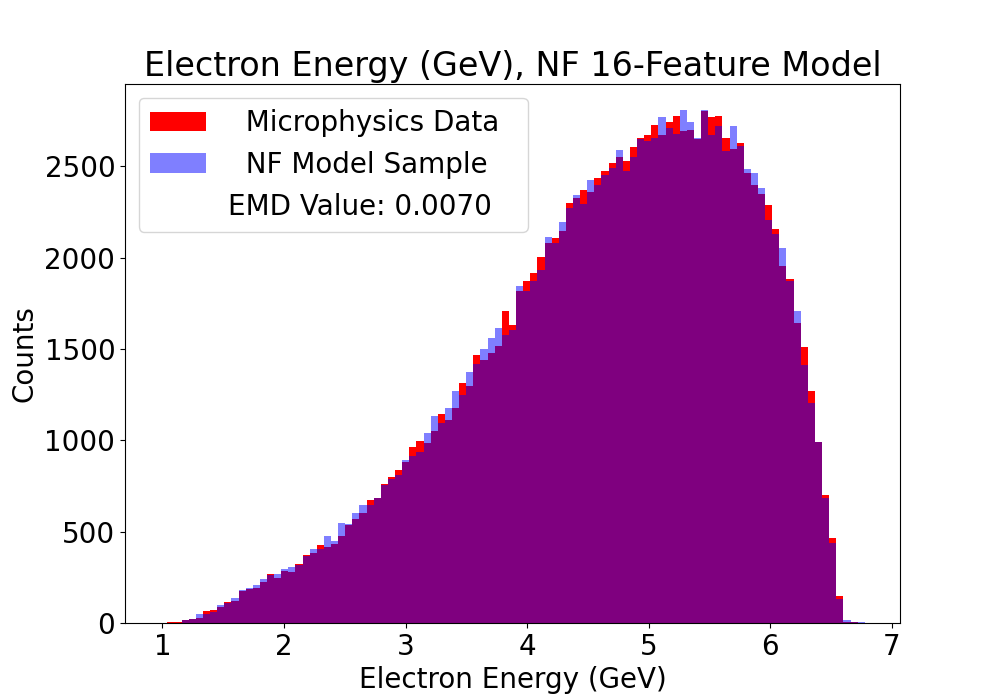
\includegraphics[width=.99\textwidth,trim={3cm 0 0 0},clip]{Chapters/Ch3-Simulations/normalizing_flows/pics/FinalPictures/Features16/Electron_Energy_,_NF_16-Feature_Model.png}
                %\caption[Placeholder Short text]{(a)}
                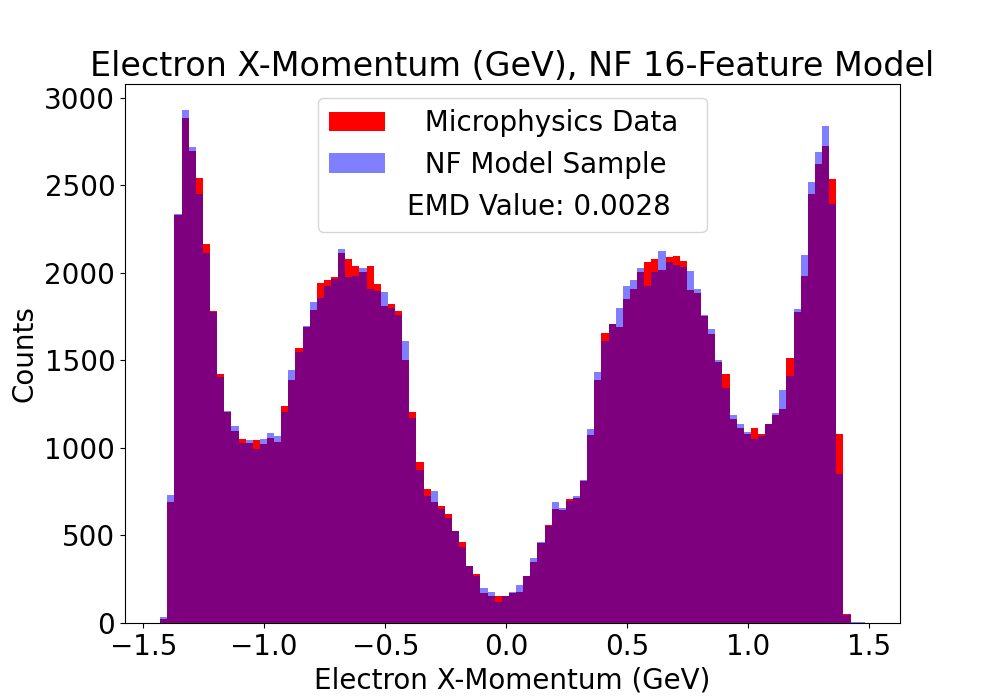
\includegraphics[width=.99\textwidth,trim={3cm 0 0 0},clip]{Chapters/Ch3-Simulations/normalizing_flows/pics/FinalPictures/Features16/Electron_X-Momentum_,_NF_16-Feature_Model.png}
                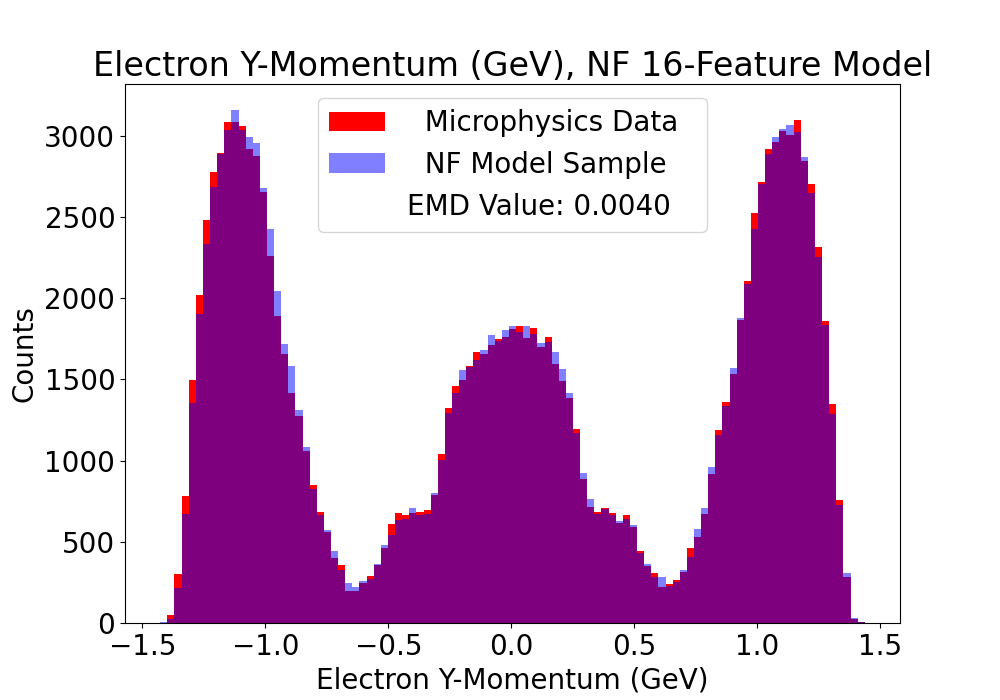
\includegraphics[width=.99\textwidth,trim={3cm 0 0 0},clip]{Chapters/Ch3-Simulations/normalizing_flows/pics/FinalPictures/Features16/Electron_Y-Momentum_,_NF_16-Feature_Model.png}
                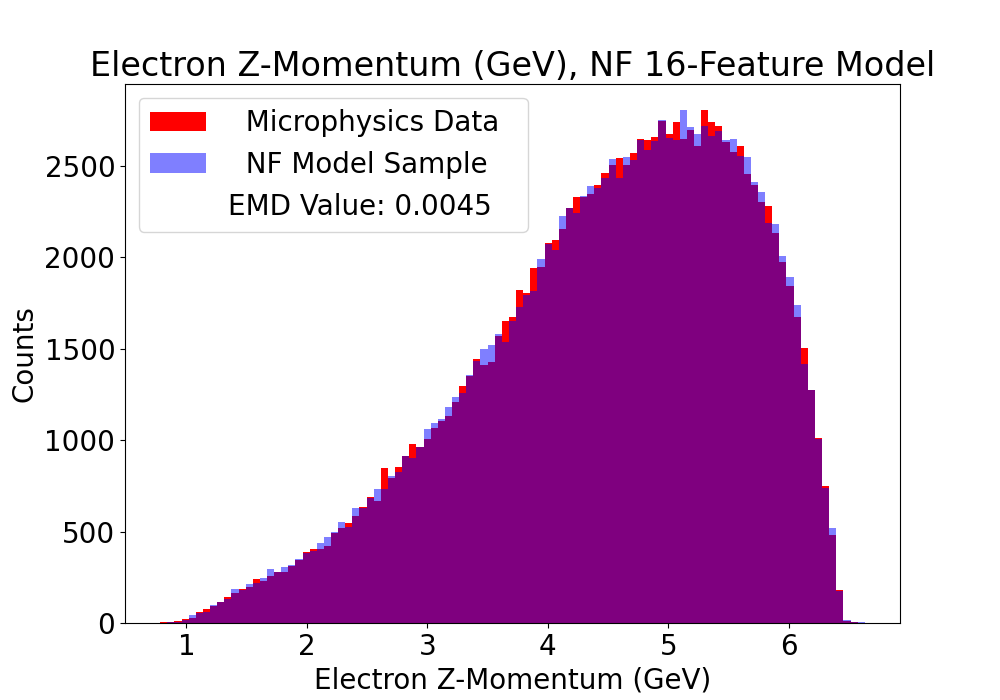
\includegraphics[width=.99\textwidth,trim={3cm 0 0 0},clip]{Chapters/Ch3-Simulations/normalizing_flows/pics/FinalPictures/Features16/Electron_Z-Momentum_,_NF_16-Feature_Model.png}
                %\caption[Placeholder Short text]{(c)}
            \end{minipage}%
            \begin{minipage}{0.23\textwidth}
                \centering
               % Proton
                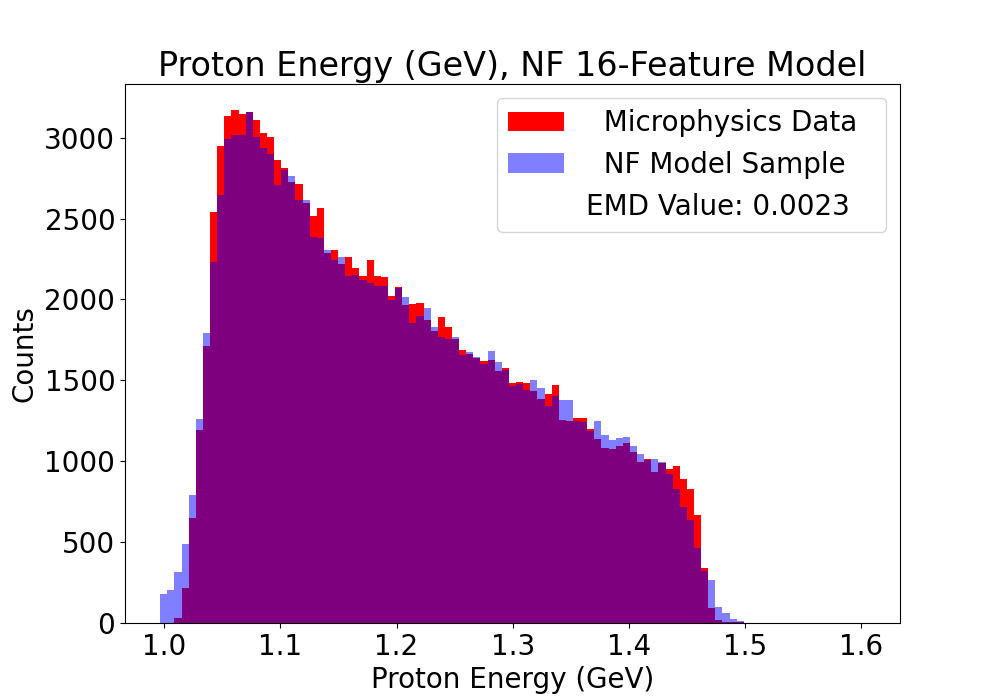
\includegraphics[width=.99\textwidth,trim={3cm 0 0 0},clip]{Chapters/Ch3-Simulations/normalizing_flows/pics/FinalPictures/Features16/Proton_Energy_,_NF_16-Feature_Model.png}
                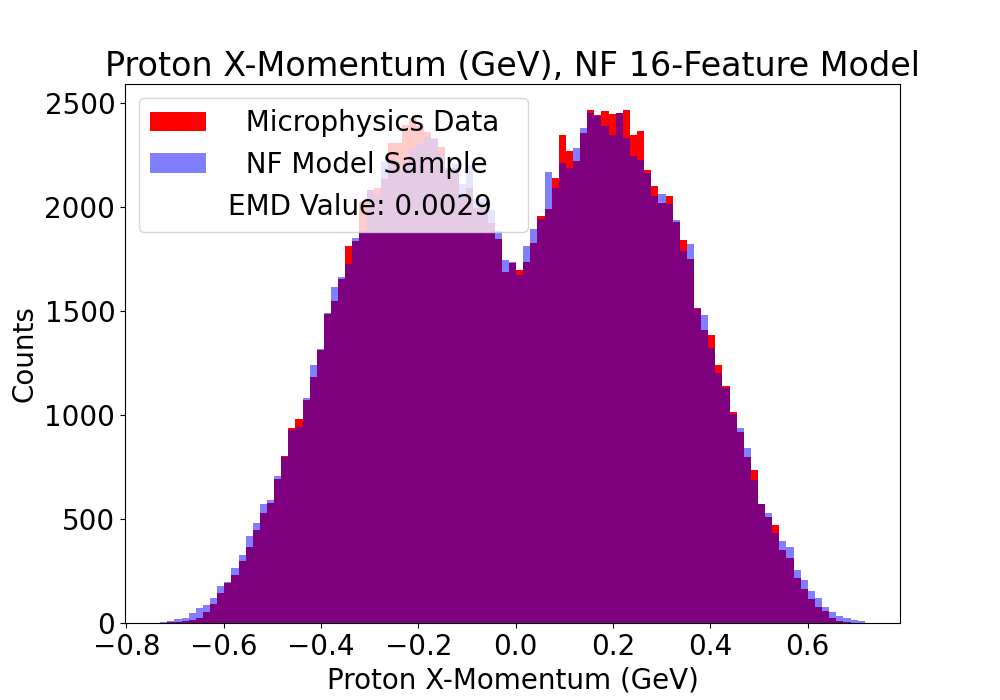
\includegraphics[width=.99\textwidth,trim={3cm 0 0 0},clip]{Chapters/Ch3-Simulations/normalizing_flows/pics/FinalPictures/Features16/Proton_X-Momentum_,_NF_16-Feature_Model.png}
                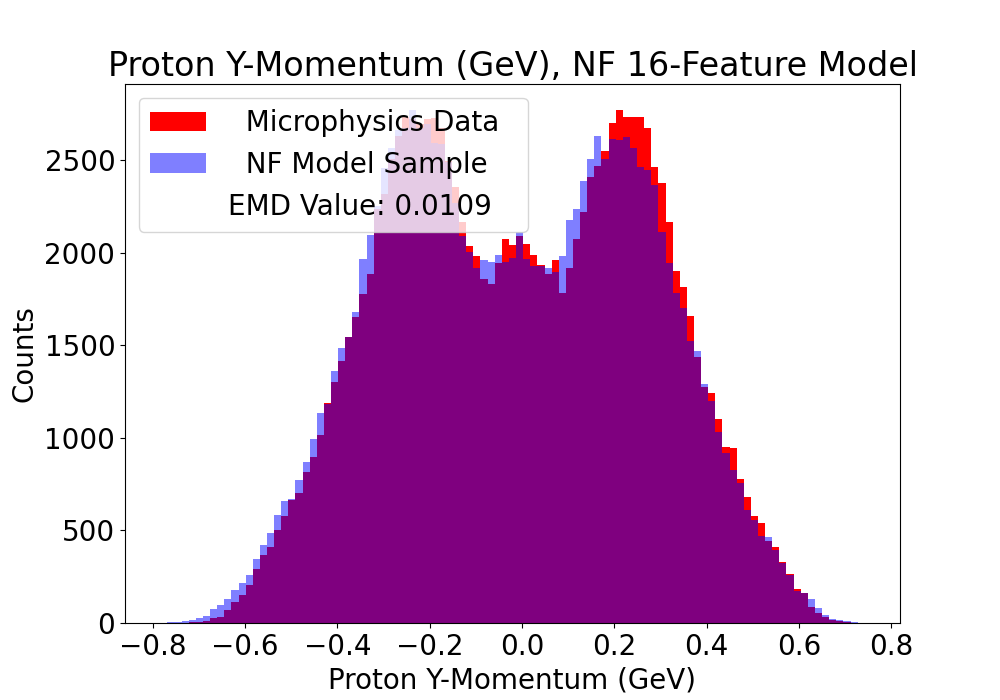
\includegraphics[width=.99\textwidth,trim={3cm 0 0 0},clip]{Chapters/Ch3-Simulations/normalizing_flows/pics/FinalPictures/Features16/Proton_Y-Momentum_,_NF_16-Feature_Model.png}
                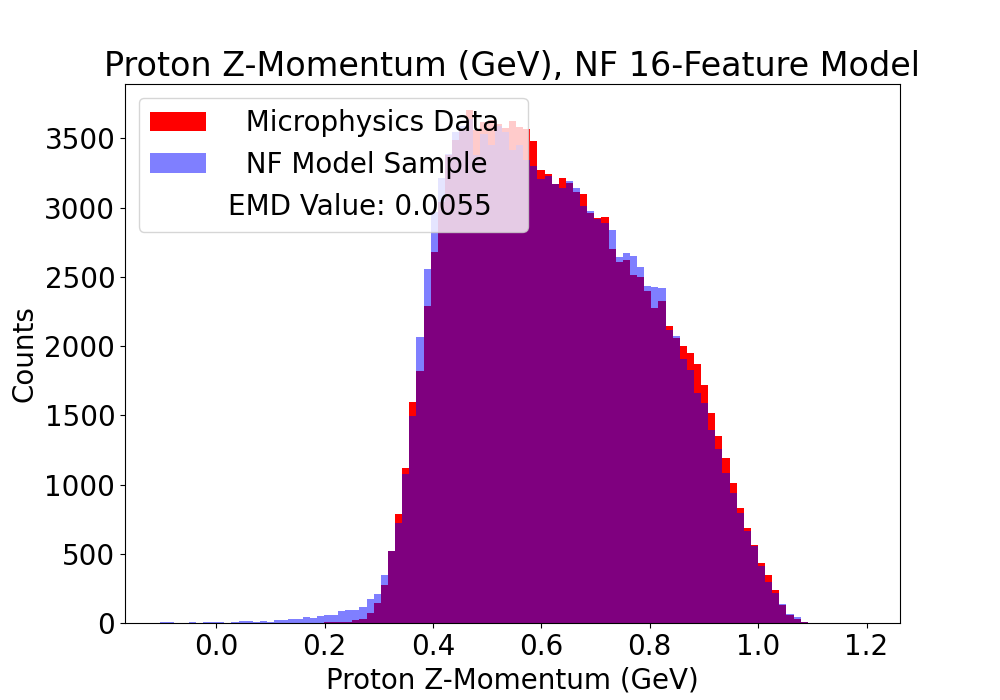
\includegraphics[width=.99\textwidth,trim={3cm 0 0 0},clip]{Chapters/Ch3-Simulations/normalizing_flows/pics/FinalPictures/Features16/Proton_Z-Momentum_,_NF_16-Feature_Model.png}
            \end{minipage}
             \begin{minipage}{0.23\textwidth}
                    \centering
                   % Photon 1
                    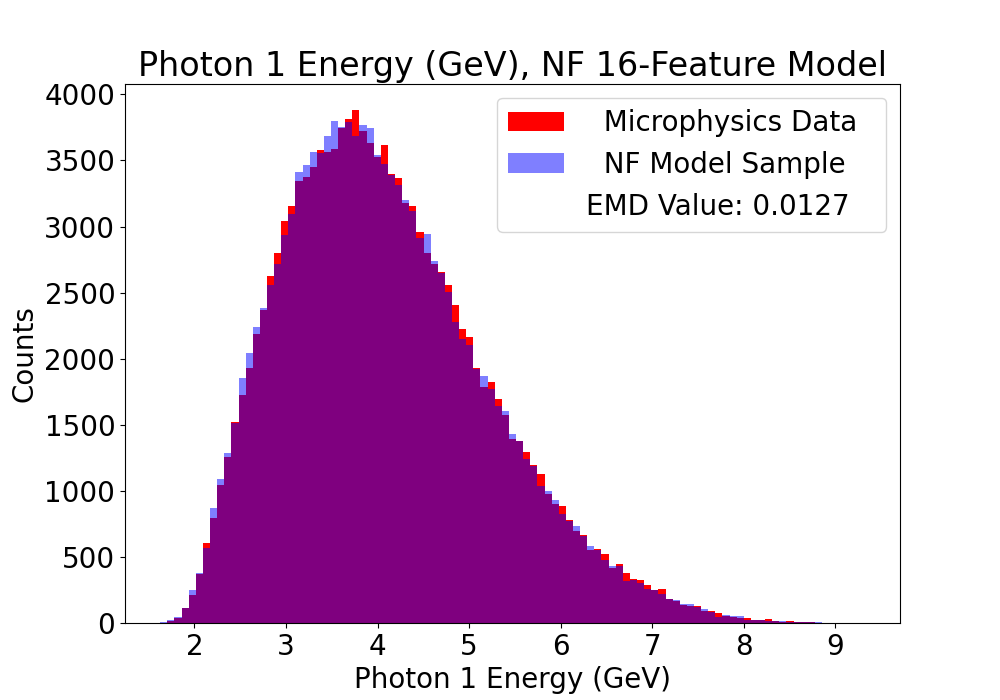
\includegraphics[width=.99\textwidth,trim={3cm 0 0 0},clip]{Chapters/Ch3-Simulations/normalizing_flows/pics/FinalPictures/Features16/Photon_1_Energy_,_NF_16-Feature_Model.png}
                    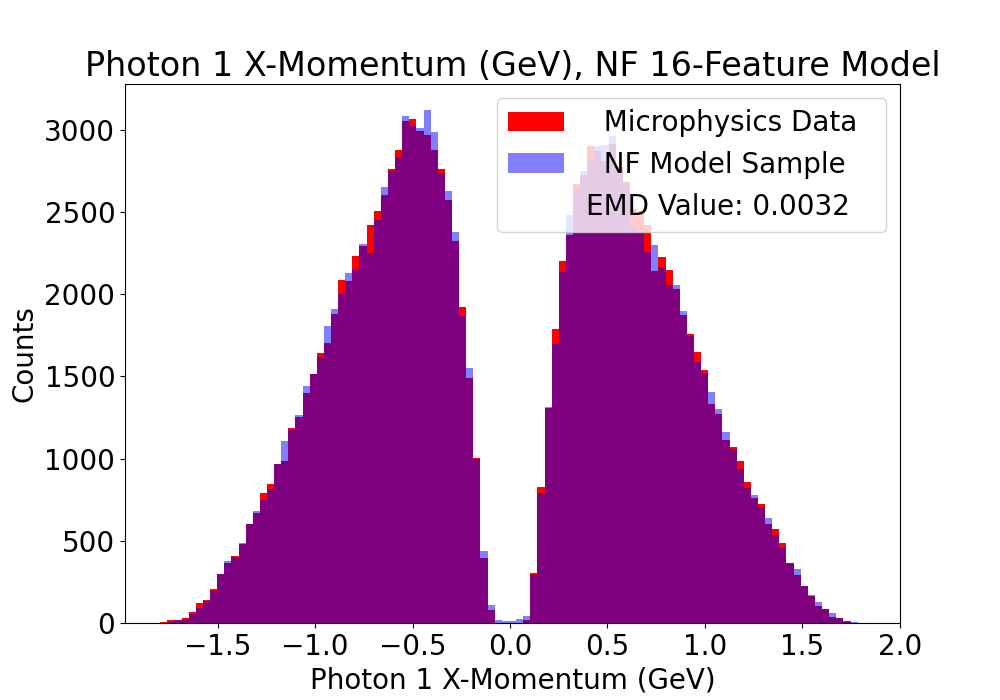
\includegraphics[width=.99\textwidth,trim={3cm 0 0 0},clip]{Chapters/Ch3-Simulations/normalizing_flows/pics/FinalPictures/Features16/Photon_1_X-Momentum_,_NF_16-Feature_Model.png}
                    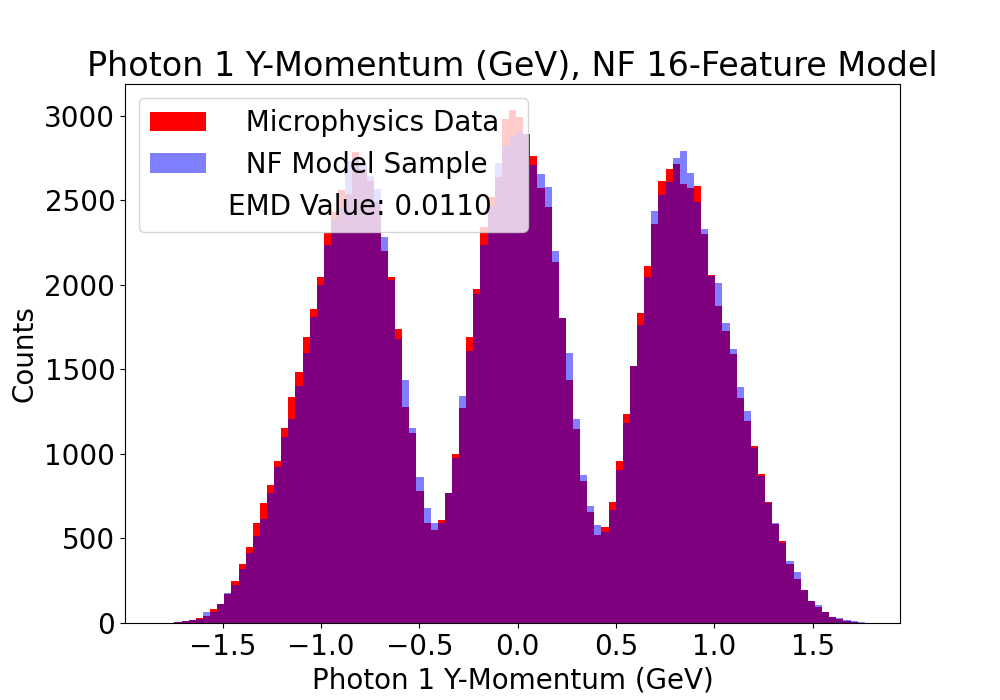
\includegraphics[width=.99\textwidth,trim={3cm 0 0 0},clip]{Chapters/Ch3-Simulations/normalizing_flows/pics/FinalPictures/Features16/Photon_1_Y-Momentum_,_NF_16-Feature_Model.png}
                    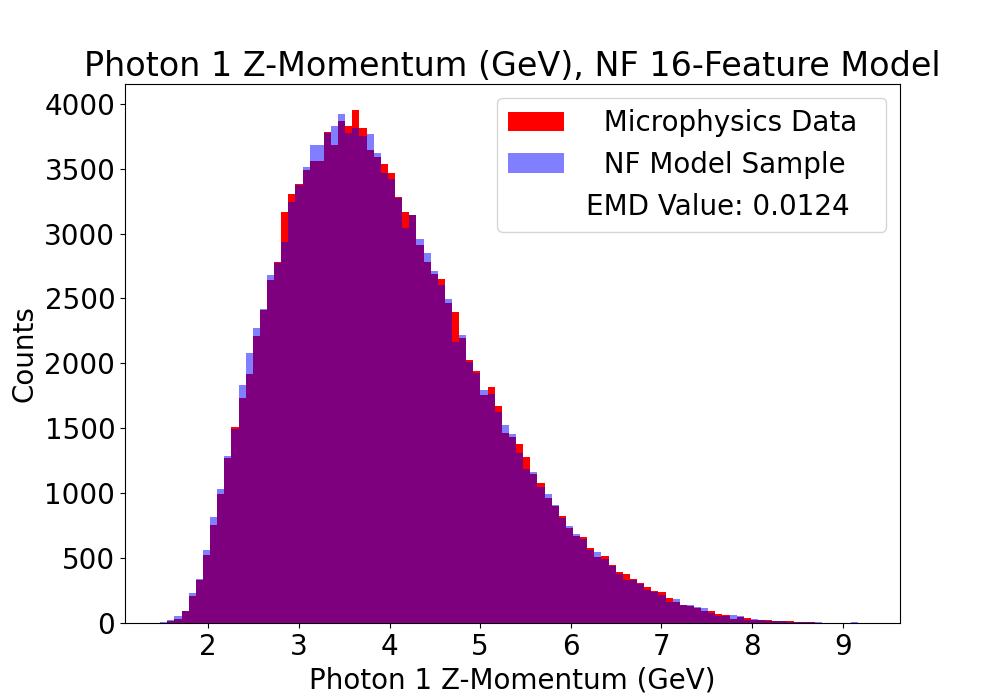
\includegraphics[width=.99\textwidth,trim={3cm 0 0 0},clip]{Chapters/Ch3-Simulations/normalizing_flows/pics/FinalPictures/Features16/Photon_1_Z-Momentum_,_NF_16-Feature_Model.png}
            \end{minipage}
             \begin{minipage}{0.23\textwidth}
                \centering
                %Photon 2
                
                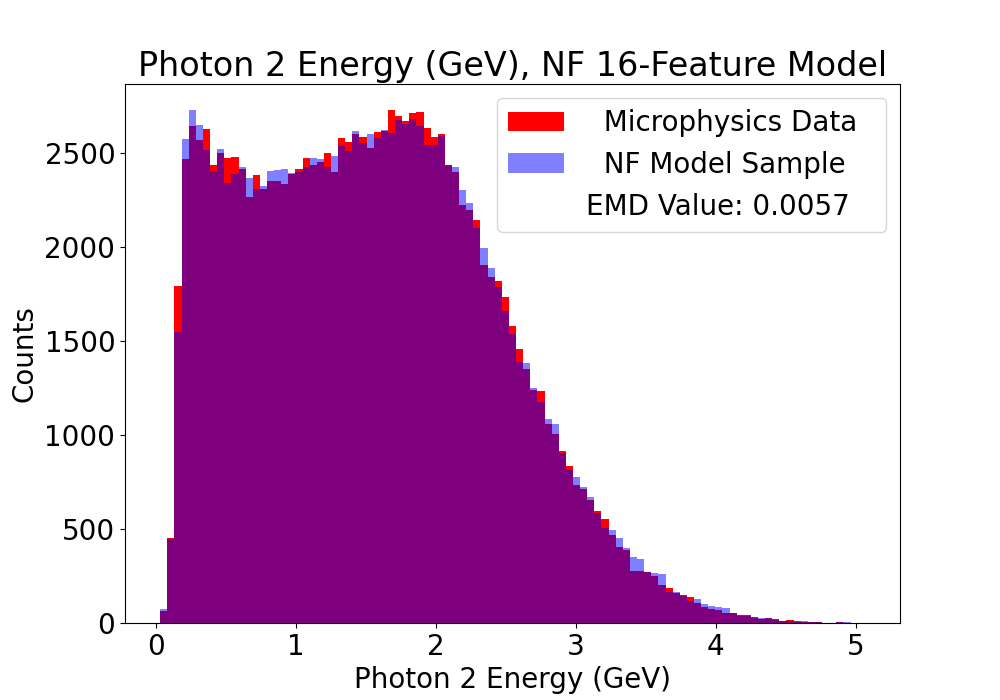
\includegraphics[width=.99\textwidth,trim={3cm 0 0 0},clip]{Chapters/Ch3-Simulations/normalizing_flows/pics/FinalPictures/Features16/Photon_2_Energy_,_NF_16-Feature_Model.png}
                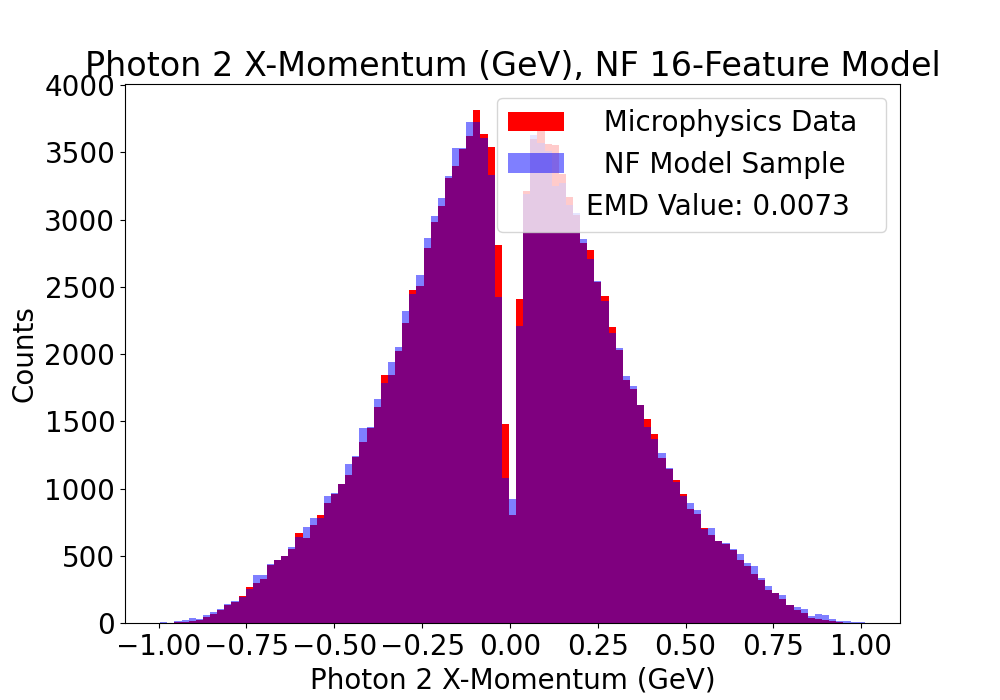
\includegraphics[width=.99\textwidth,trim={3cm 0 0 0},clip]{Chapters/Ch3-Simulations/normalizing_flows/pics/FinalPictures/Features16/Photon_2_X-Momentum_,_NF_16-Feature_Model.png}
                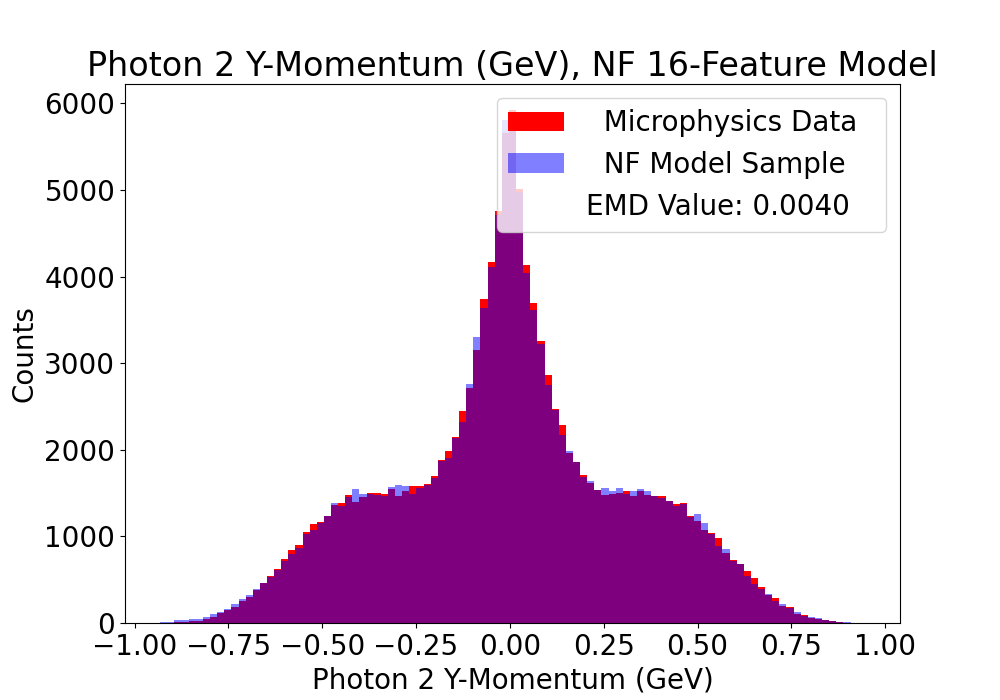
\includegraphics[width=.99\textwidth,trim={3cm 0 0 0},clip]{Chapters/Ch3-Simulations/normalizing_flows/pics/FinalPictures/Features16/Photon_2_Y-Momentum_,_NF_16-Feature_Model.png}
                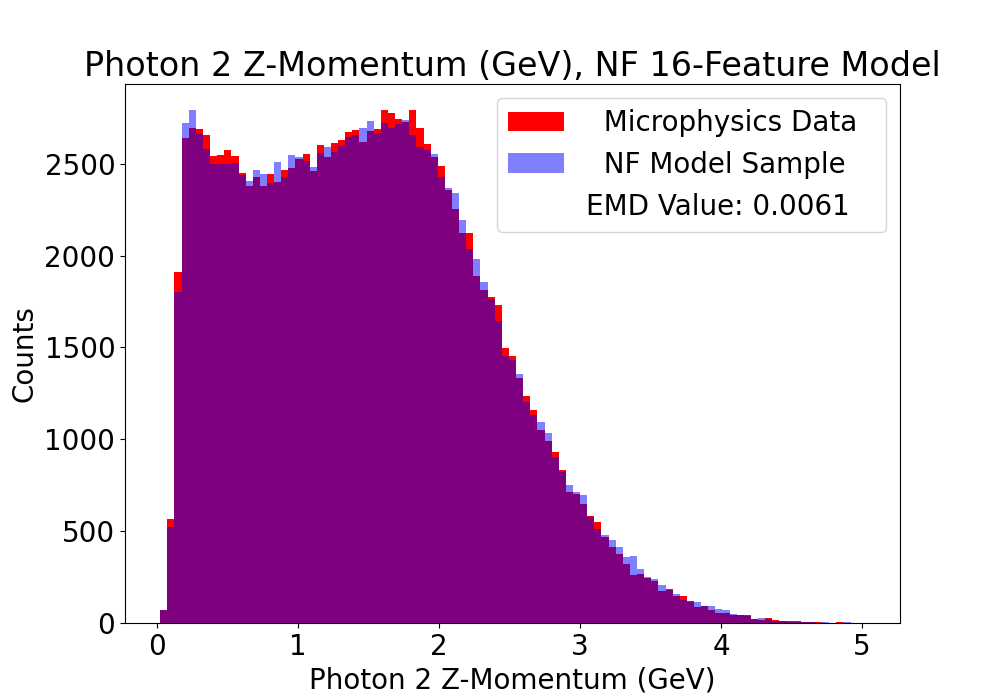
\includegraphics[width=.99\textwidth,trim={3cm 0 0 0},clip]{Chapters/Ch3-Simulations/normalizing_flows/pics/FinalPictures/Features16/Photon_2_Z-Momentum_,_NF_16-Feature_Model.png}
            \end{minipage}
            \caption[Placeholder Short text]{The 1D distributions of all 16 features sampled from our NF model (blue), and from physics simulation (red). Each histogram is normalized to the area, and has 100 bins.}
            \label{fig:16features}
        \end{figure}
        
        
        
        \begin{figure}[H]
            \centering
            %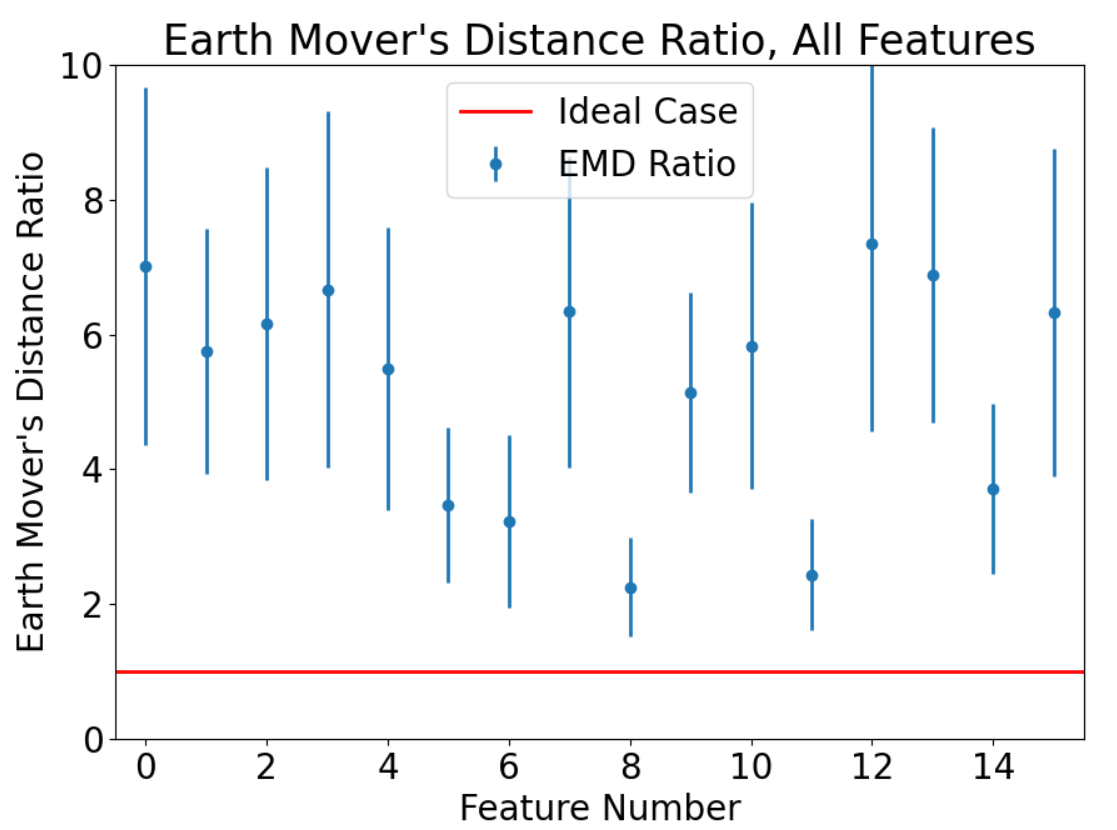
\includegraphics[scale=0.3]{FinalPictures/EMD/EmdRatio.png}
            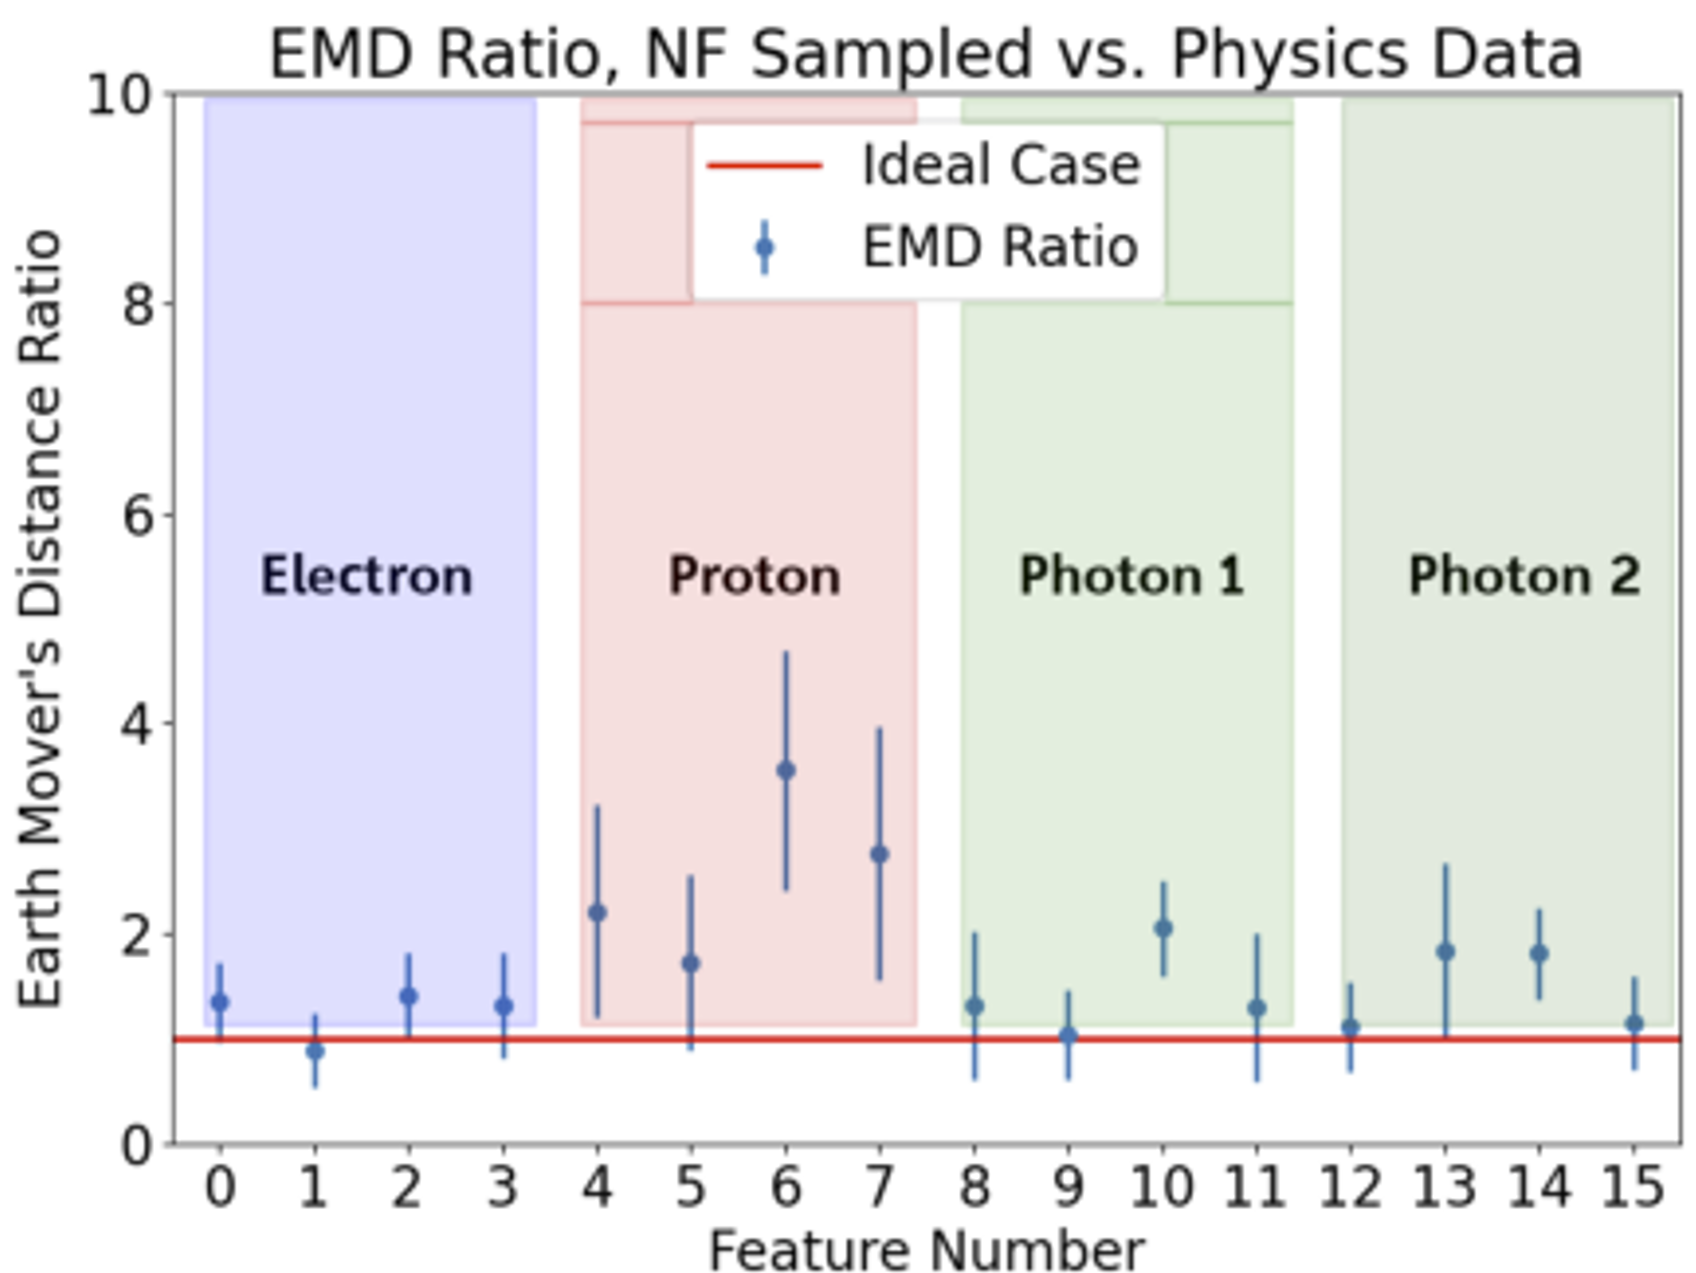
\includegraphics[width=.8\textwidth,trim={0 0 0 0 },clip]{Chapters/Ch3-Simulations/normalizing_flows/pics/FinalPictures/EMD/EMD_updated.png}
            \caption[Placeholder Short text]{The EMD ratios of all 16 features between the NF generated distributions and sample from physics simulation. The points are the average EMD ratios of 10 different subsample calculations; the error bars are the standard deviations of the sets. If the model were perfect, all points would have value 1; deviation from 1 indicates worse performance.}
            \label{fig:EMD}
        \end{figure}
        
        To understand the shortcomings of the trained model, we consider 2-Dimensional distributions in  Figure \ref{fig:2D}. We can see that while some distributions are reproduced well, the fine detail and hard cutoffs that exist in some feature spaces are not learned sharply by the model and result in haziness. Specifically, only certain combinations of particle momenta are measurable due to the physical limitations of our real-world detectors (and hence, our computer-modeled detectors in the traditional microphysics simulations) as well as due to physics conservation law constraints. However, we have yet to incorporate these constraints into our NF model training, and so the samples generated from this trained model exist in traditionally empty regions of phase space. One solution to this issue is to implement filtering after sampling from the model, but given the already slow sampling rate, this would further decrease the speed advantage offered by the normalizing flow method. Work is ongoing to incorporate these constraints in the training of the model itself.
        
        \begin{figure}[H]
            \centering
            \begin{minipage}{.3133\textwidth}
            
                \centering
               % Electron
                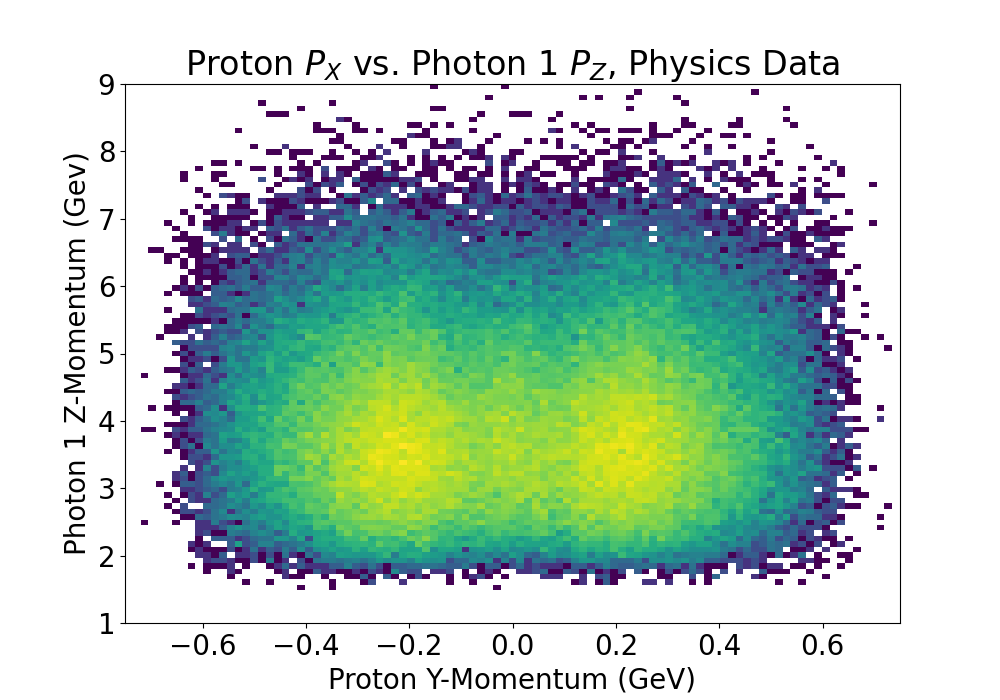
\includegraphics[width=.99\textwidth,trim={0 0 0 0},clip]{Chapters/Ch3-Simulations/normalizing_flows/pics/FinalPictures/Hists2D/Proton_P_X_vs_Photon_1_P_Z,_Physics_Data.png}
                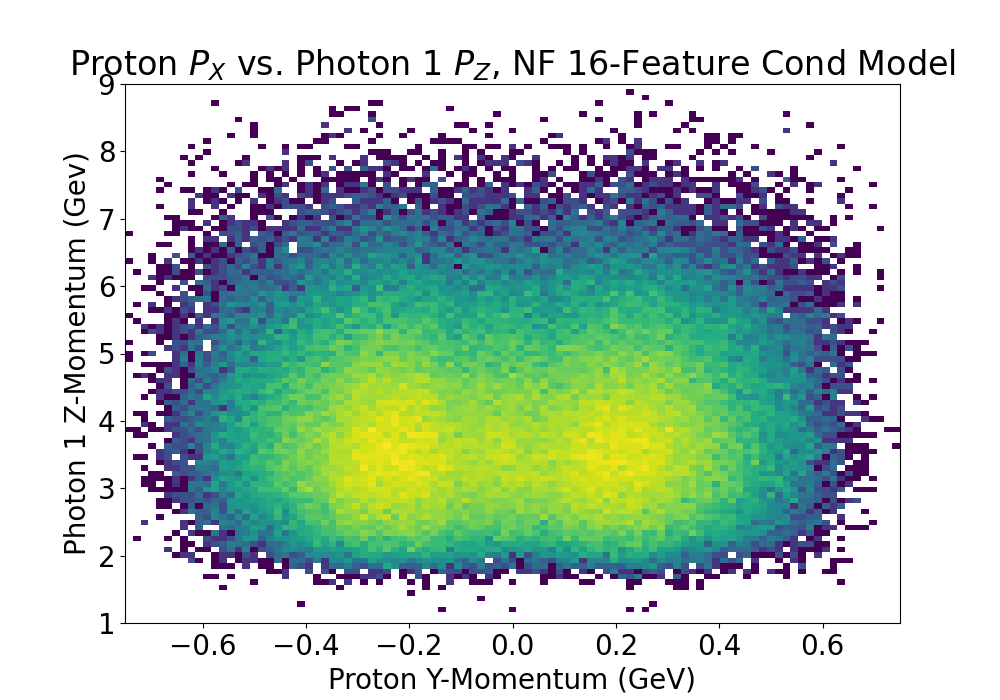
\includegraphics[width=.99\textwidth,trim={0 0 0 0},clip]{Chapters/Ch3-Simulations/normalizing_flows/pics/FinalPictures/Hists2D/Proton_P_X_vs_Photon_1_P_Z,_NF_16-Feature_Cond_Model.png}
        
                %\caption[Placeholder Short text]{(c)}
            \end{minipage}%
            \begin{minipage}{0.3133\textwidth}
                \centering
               %Feature Distributions from Traditional Microphysics Simulations
                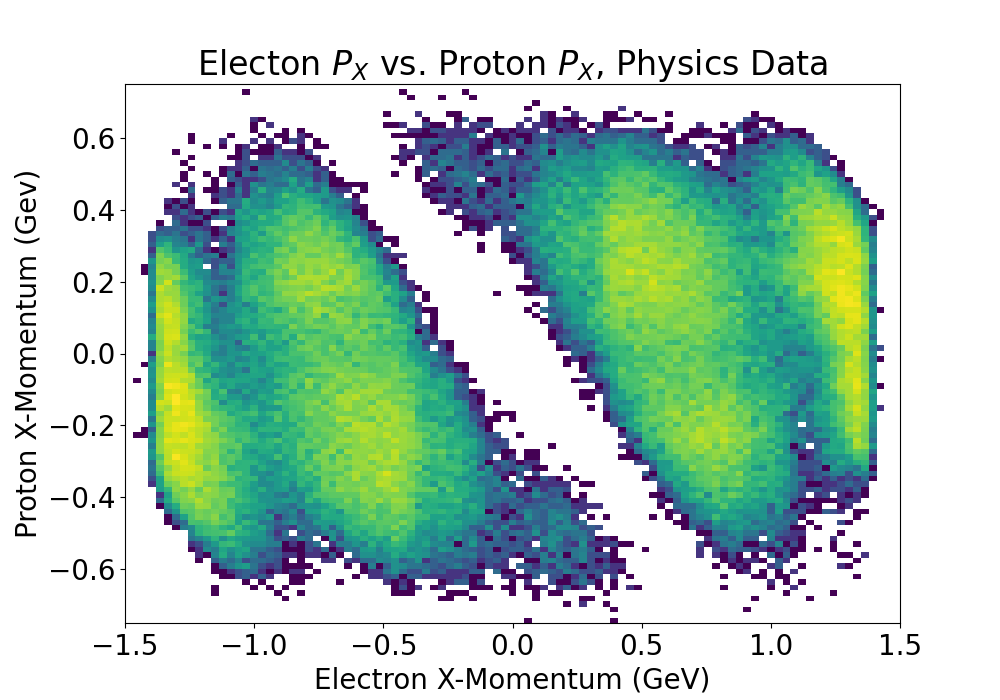
\includegraphics[width=.99\textwidth,trim={0 0 0 0},clip]{Chapters/Ch3-Simulations/normalizing_flows/pics/FinalPictures/Hists2D/Electon_P_X_vs_Proton_P_X,_Physics_Data.png}
                %Feature Distributions from NF Model Samples
                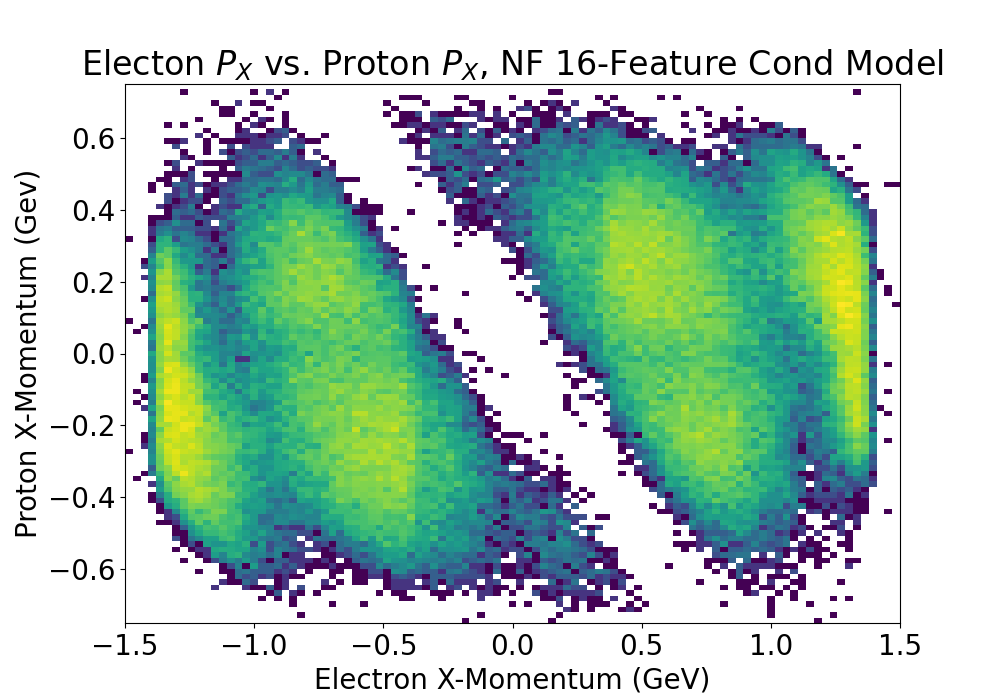
\includegraphics[width=.99\textwidth,trim={0 0 0 0},clip]{Chapters/Ch3-Simulations/normalizing_flows/pics/FinalPictures/Hists2D/Electon_P_X_vs_Proton_P_X,_NF_16-Feature_Cond_Model.png}
                %\caption[Placeholder Short text]{(a)}
                
        
            \end{minipage}
             \begin{minipage}{0.3133\textwidth}
                    \centering
                   % Photon 1
                    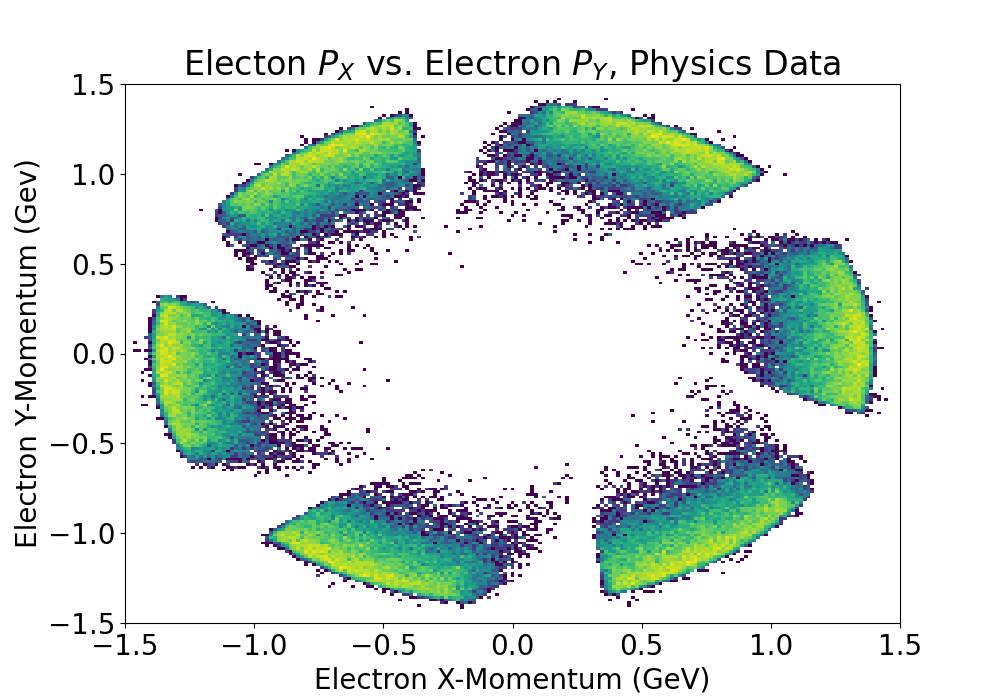
\includegraphics[width=.99\textwidth,trim={0 0 0 0},clip]{Chapters/Ch3-Simulations/normalizing_flows/pics/FinalPictures/Hists2D/Electon_P_X_vs_Electron_P_Y,_Physics_Data.png}
                    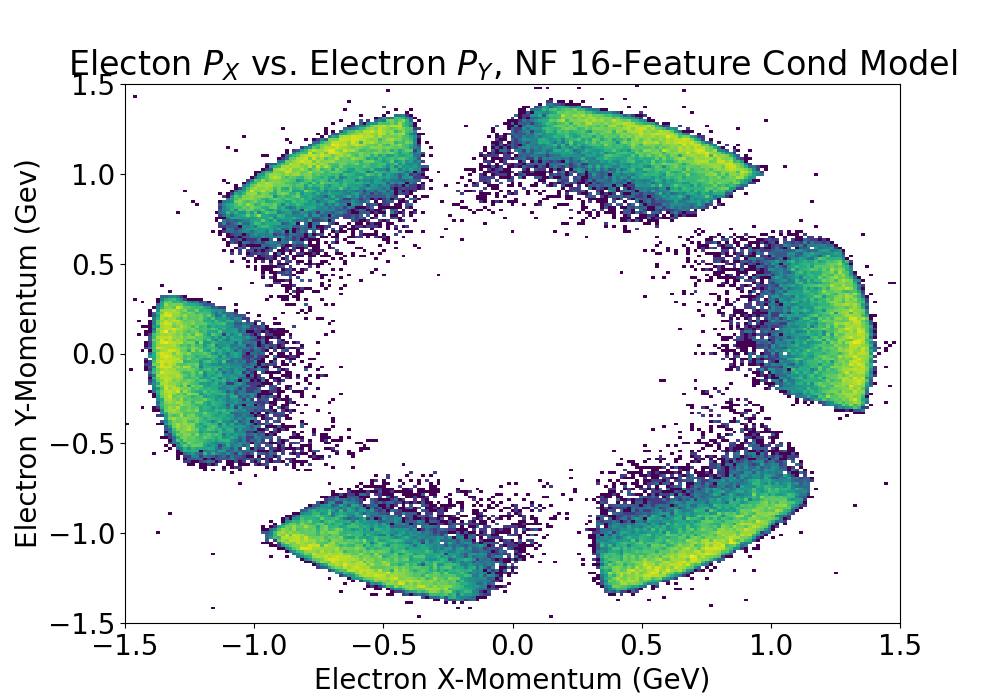
\includegraphics[width=.99\textwidth,trim={0 0 0 0},clip]{Chapters/Ch3-Simulations/normalizing_flows/pics/FinalPictures/Hists2D/Electon_P_X_vs_Electron_P_Y,_NF_16-Feature_Cond_Model.png}
        
            \end{minipage}
            \caption[Placeholder Short text]{ 2-Dimensional distributions for various features, comparing the data from the traditional physics simulation to the NF sampled data. \textbf{Top} Feature distributions from the traditional physics data set. \textbf{Bottom} Feature distributions from our trained NF model, which should match with the top row. Moving from left to right, we can see that some feature distributions are reproduced well, while others have difficult details that are not well modeled, corresponding to physical detector geometry and physics constraints that the NF model is unaware of. }
            \label{fig:2D}
        \end{figure}
        
        
        To try to improve fine-detail reproduction by our model, we trained a second model with only 4-features, which corresponded to a full description of a simulated electron. We observed some improvement in the fidelity of feature reproduction, in particular, Figure \ref{fig:EMD2} shows that, compared to the 16-feature trained model, the 4-feature model (trained only on electron features) exhibits a 2-4 times lower EMD. Of course, this 4-feature trained model is much more limited in scope, but also is able to produce samples much faster, at a rate of about 170 Hz, compared to 4 Hz for the 16-feature model. Given that it describes fully a simulated electron, this would be useful for generally speeding up simulations, but the correlations between different particles that define specific processes like DV$\pi$P is lost. 
        
        
        \begin{figure}[H]
            \centering
            %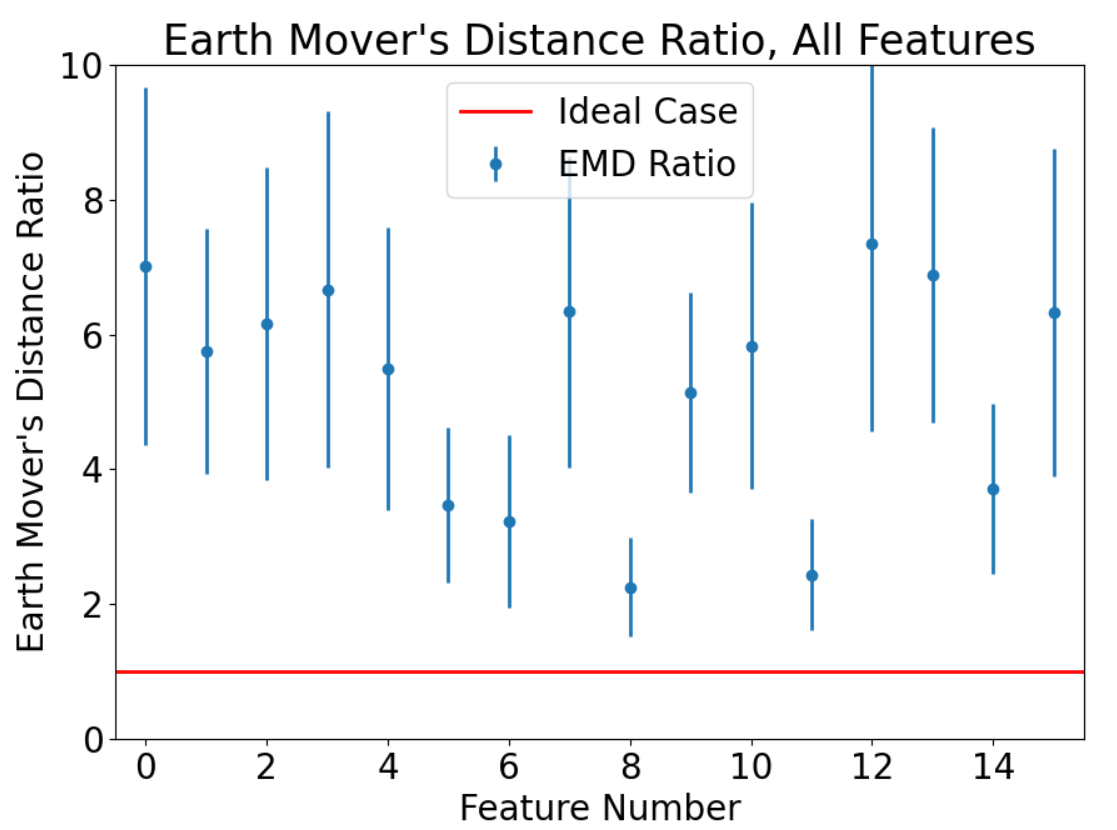
\includegraphics[scale=0.3]{FinalPictures/EMD/EmdRatio.png}
            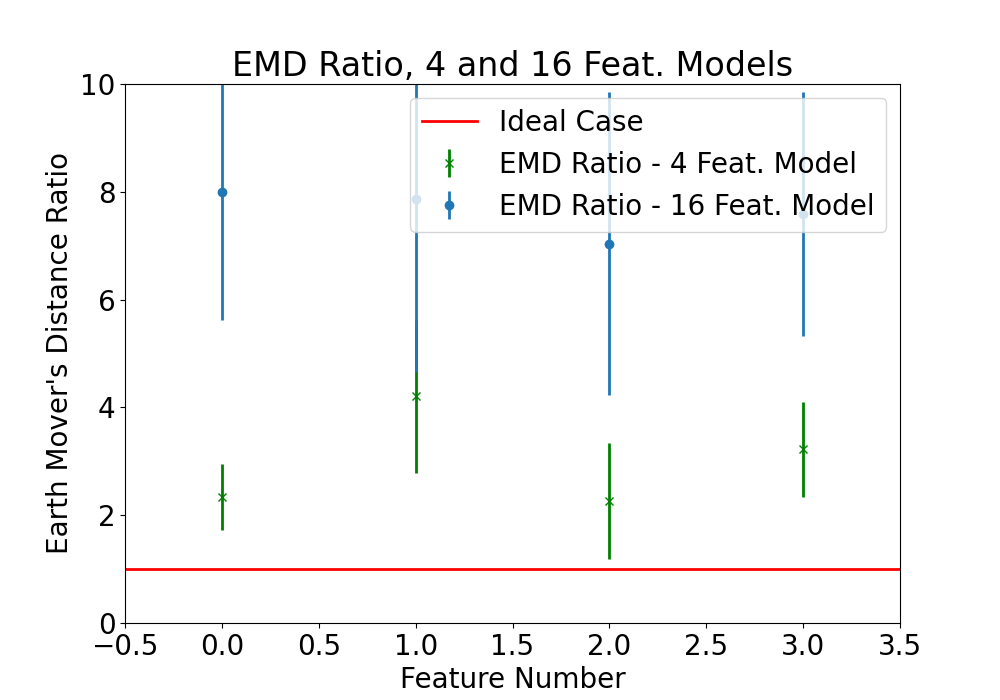
\includegraphics[width=.47\textwidth,trim={ 0 0 0 0},clip]{Chapters/Ch3-Simulations/normalizing_flows/pics/FinalPictures/EMD/emdratio416.png}
            \caption[Placeholder Short text]{The EMD Ratio of selected 4 features between the NF generated distributions and sample from physics simulation when the model was trained using all 16 features as Fig.~\ref{fig:EMD} (blue), and the selected 4 features (green). The 4-Feature trained model shows consistently lower EMD ratio values than the 16-trained model, indicating a better ability to reproduce electron features.}
            \label{fig:EMD2}
        \end{figure}
        
        Comparing to Figure \ref{fig:2D}, we can see from Figure \ref{fig:2D4F} that the 4-feature trained NF model also demonstrates better reproduction of the sharp cutoffs in distributions caused by detector and physics constraints, although still the match is not perfect. Work is ongoing to directly include these constraints in the NF training to decrease these discrepancies.
        
        \begin{figure}[H]
            \centering
             \begin{minipage}{0.31323\textwidth}
                \centering
                Traditional Simulation
                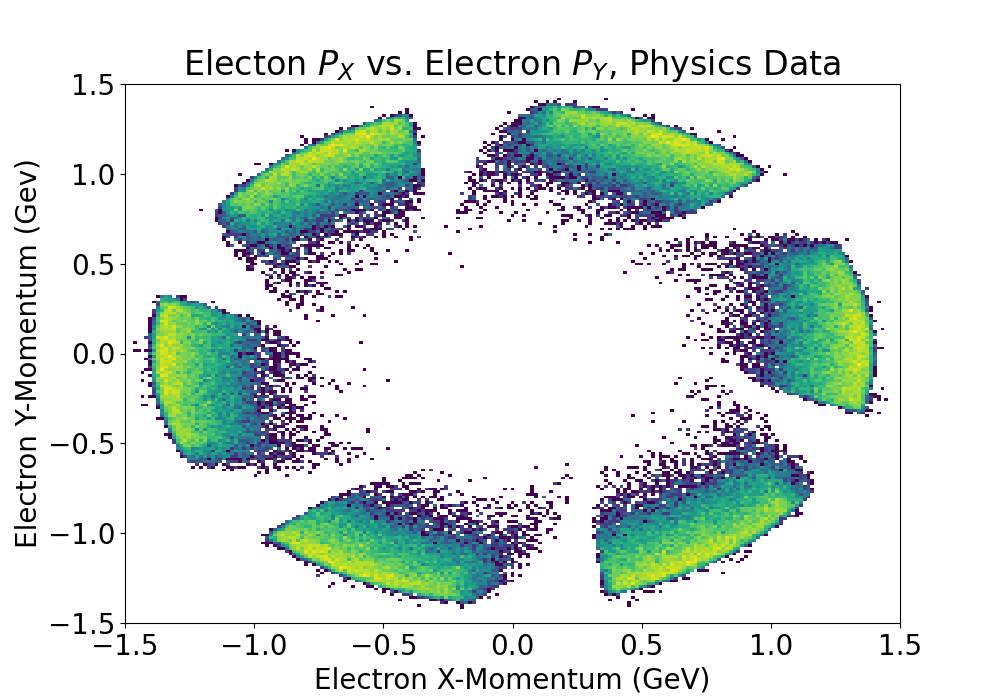
\includegraphics[width=.99\textwidth,trim={0 0 0 0},clip]{Chapters/Ch3-Simulations/normalizing_flows/pics/FinalPictures/Hists2D/Electon_P_X_vs_Electron_P_Y,_Physics_Data.png}
                
            \end{minipage}
                 \begin{minipage}{0.31323\textwidth}
                \centering
                16-Feature Model
                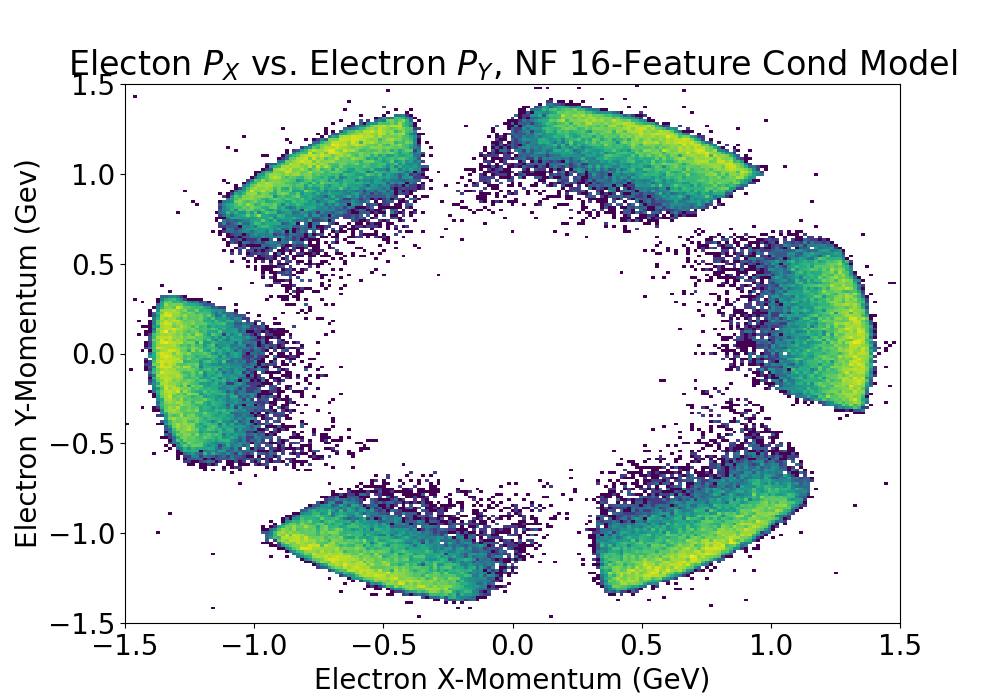
\includegraphics[width=.99\textwidth,trim={0 0 0 0},clip]{Chapters/Ch3-Simulations/normalizing_flows/pics/FinalPictures/Hists2D/Electon_P_X_vs_Electron_P_Y,_NF_16-Feature_Cond_Model.png}
        
            \end{minipage}
                 \begin{minipage}{0.31323\textwidth}
                \centering
                4-Feature\\ Model
               
                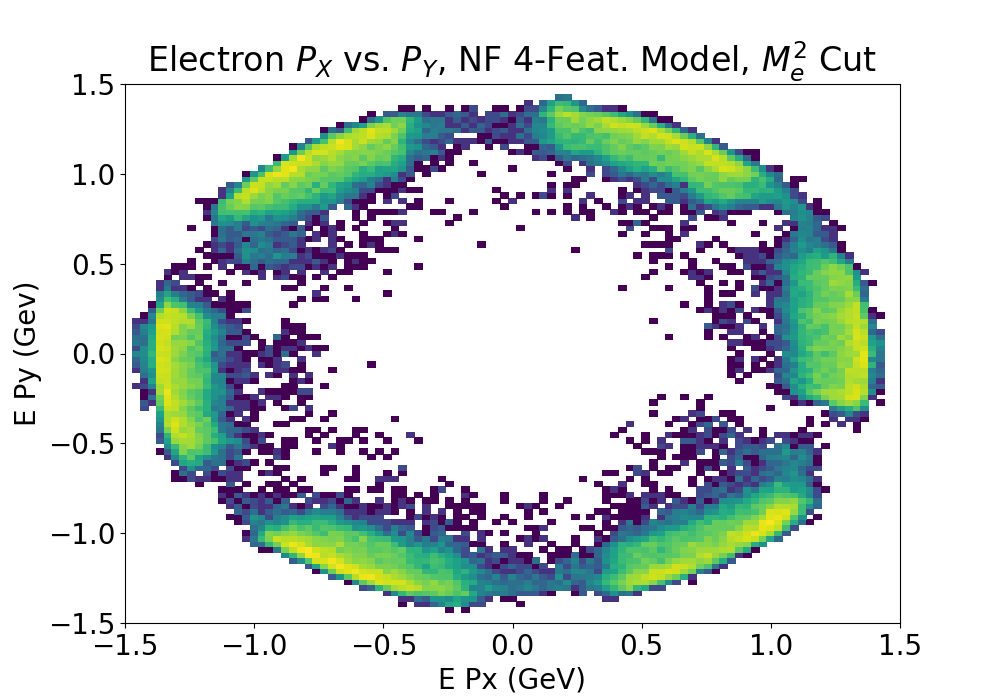
\includegraphics[width=.99\textwidth,trim={0 0 0 0},clip]{Chapters/Ch3-Simulations/normalizing_flows/pics/FinalPictures/2D_Hists_4F/Electron_P_X_vs_P_Y,_NF_4-Feat_Model,_M_e2_Cut.png}
            \end{minipage}
            \caption[Placeholder Short text]{\textbf{Left}: Electron X-Momentum vs. Electron Y-Momentum distribution from the traditional physics simulation dataset. \textbf{Center}: The observed distribution from the 16-Feature trained model, copied from Figure \ref{fig:2D} for reference. We can see considerable disparity between this distribution and the traditional physics distribution. \textbf{Right}: The distribution result from the 4-Feature trained model, which demonstrates far greater agreement to the traditional results compared to the 16-Feature model. }
            \label{fig:2D4F}
        \end{figure}
        
        
        Ultimately, we are interested in physics processes rather than just distribution mapping, so we also examined our ability to reconstruct physics quantities from the trained NF model sample data. Figure \ref{fig:protonspions} shows the distribution of calculated proton and pion (calculated from a combination of the photon features) masses from our NF model data, which had no explicit physics constraints in training. We observe a peak at about 0.939 GeV for the proton and 0.136 GeV for the pion, , which is within 0.5\% of the value encapsulated in the traditional physics training dataset. 
        
        
        \begin{figure}[H]
            \centering
            %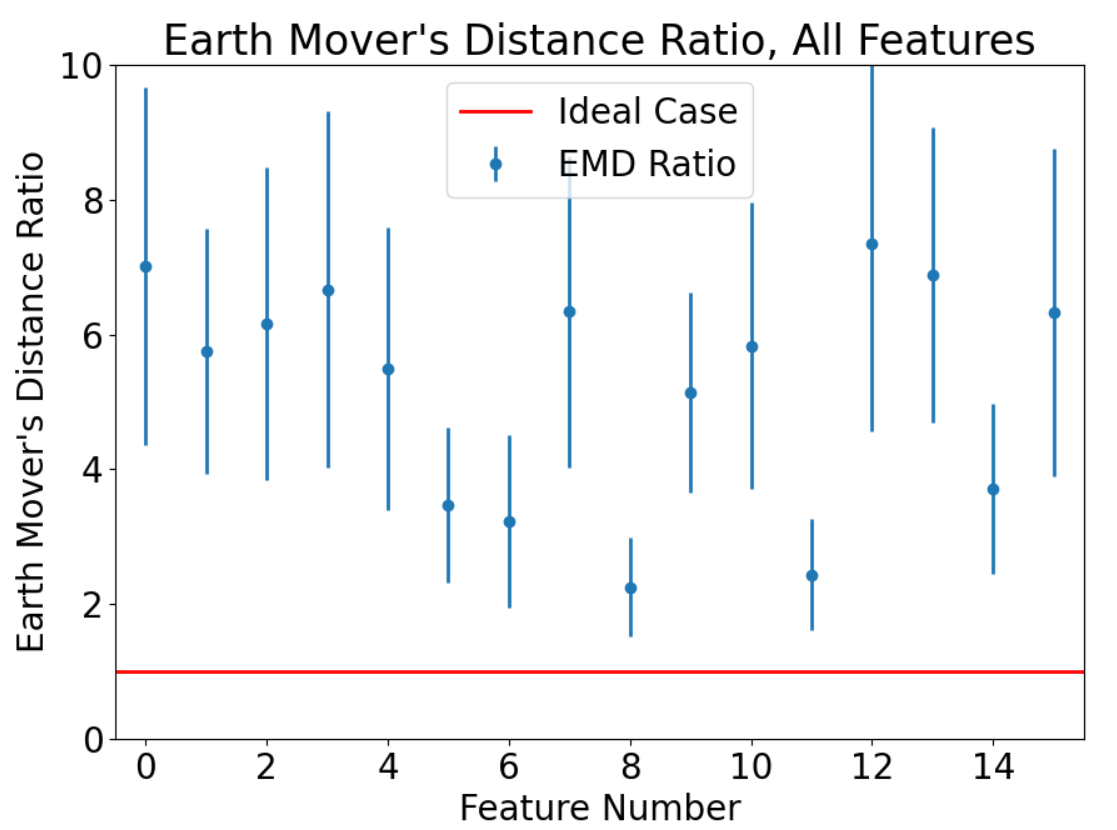
\includegraphics[scale=0.3]{FinalPictures/EMD/EmdRatio.png}
            \label{fig:protons}
        \end{figure}
        
        
        \begin{figure}[H]
            \centering
             \begin{minipage}{0.42349\textwidth}
                \centering
                %Photon 2
                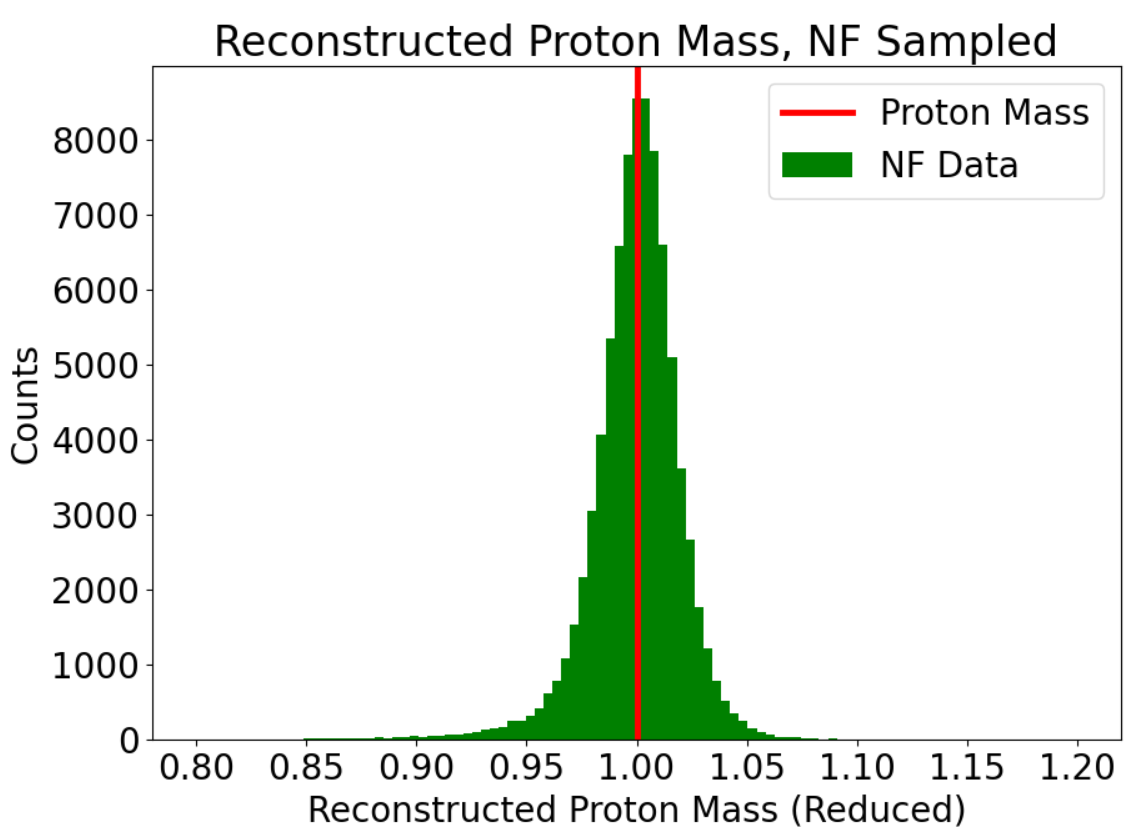
\includegraphics[width=.97\textwidth,trim={ 0 0 0 0},clip]{Chapters/Ch3-Simulations/normalizing_flows/pics/FinalPictures/updated_proton_reduced.png}
        
            \end{minipage}
            \begin{minipage}{0.421245\textwidth}
                \centering
                %Photon 2
                
                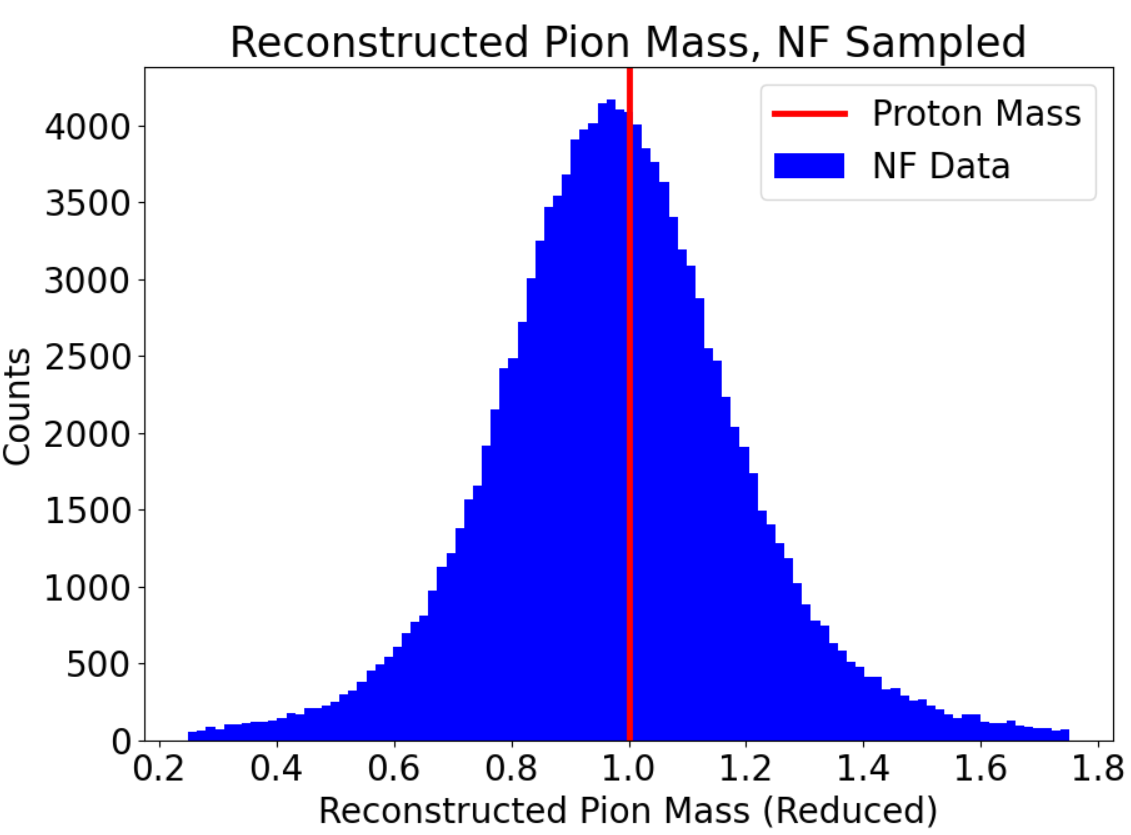
\includegraphics[width=.97\textwidth,trim={ 0 0 0 0},clip]{Chapters/Ch3-Simulations/normalizing_flows/pics/FinalPictures/updated_pion_reduced.png}
            \end{minipage}
                \caption[Placeholder Short text]{The distributions of calculated proton mass (left) and pion mass (right) from the 16-Feature trained NF model.  The accepted (true) particle masses are indicated by the red vertical lines, at 0.938 GeV and 0.135 GeV, respectively.
                The peaks from the model are about 1 MeV, or about 0.5\%, shifted away from these true values; while this is small, it is currently unclear what is causing this shift.}
            \label{fig:protonspions}
        \end{figure}
        
        
        Overall, we are able to use a UMNN-MAF architecture to attain reasonable physics distributions far faster than just using traditional physics simulations. At this stage, it is not clear if the 10x speedup afforded by the 16-feature NF model is sufficiently large to justify a decrease in fine-detail resolution. Work is ongoing as to if the model resolution can be improved by including conservation laws as part of training, or if the model can be optimized to generate samples faster. 
        
        On the other hand, the 4-feature model has both higher resolution, and is able to produce samples 1,000 times faster than traditional methods, and so could be very useful immediately to physics research efforts. However, as it is only 4-features, it can only represent one particle, not an entire physics process, but this is still relevant to the study of background processes and noise events in physics experiments, and we are investigating applying this to current CLAS12 research.
        
        The ability of the 16-Feature model to produce realistic protons and pions demonstrates viability for using this method in real physics analysis, but we show there are fine details that the model cannot learn without additional constraints. Work is ongoing to incorporate the physical experimental layout and physics conservation laws into the flow training, which we expect will resolve these discrepancies in fine-detail reproduction, and will lead to a more accurate reproduction of the traditional simulation results, at a far faster speed. 

        \begin{figure}[H]
            \centering
            \subfloat[]{
            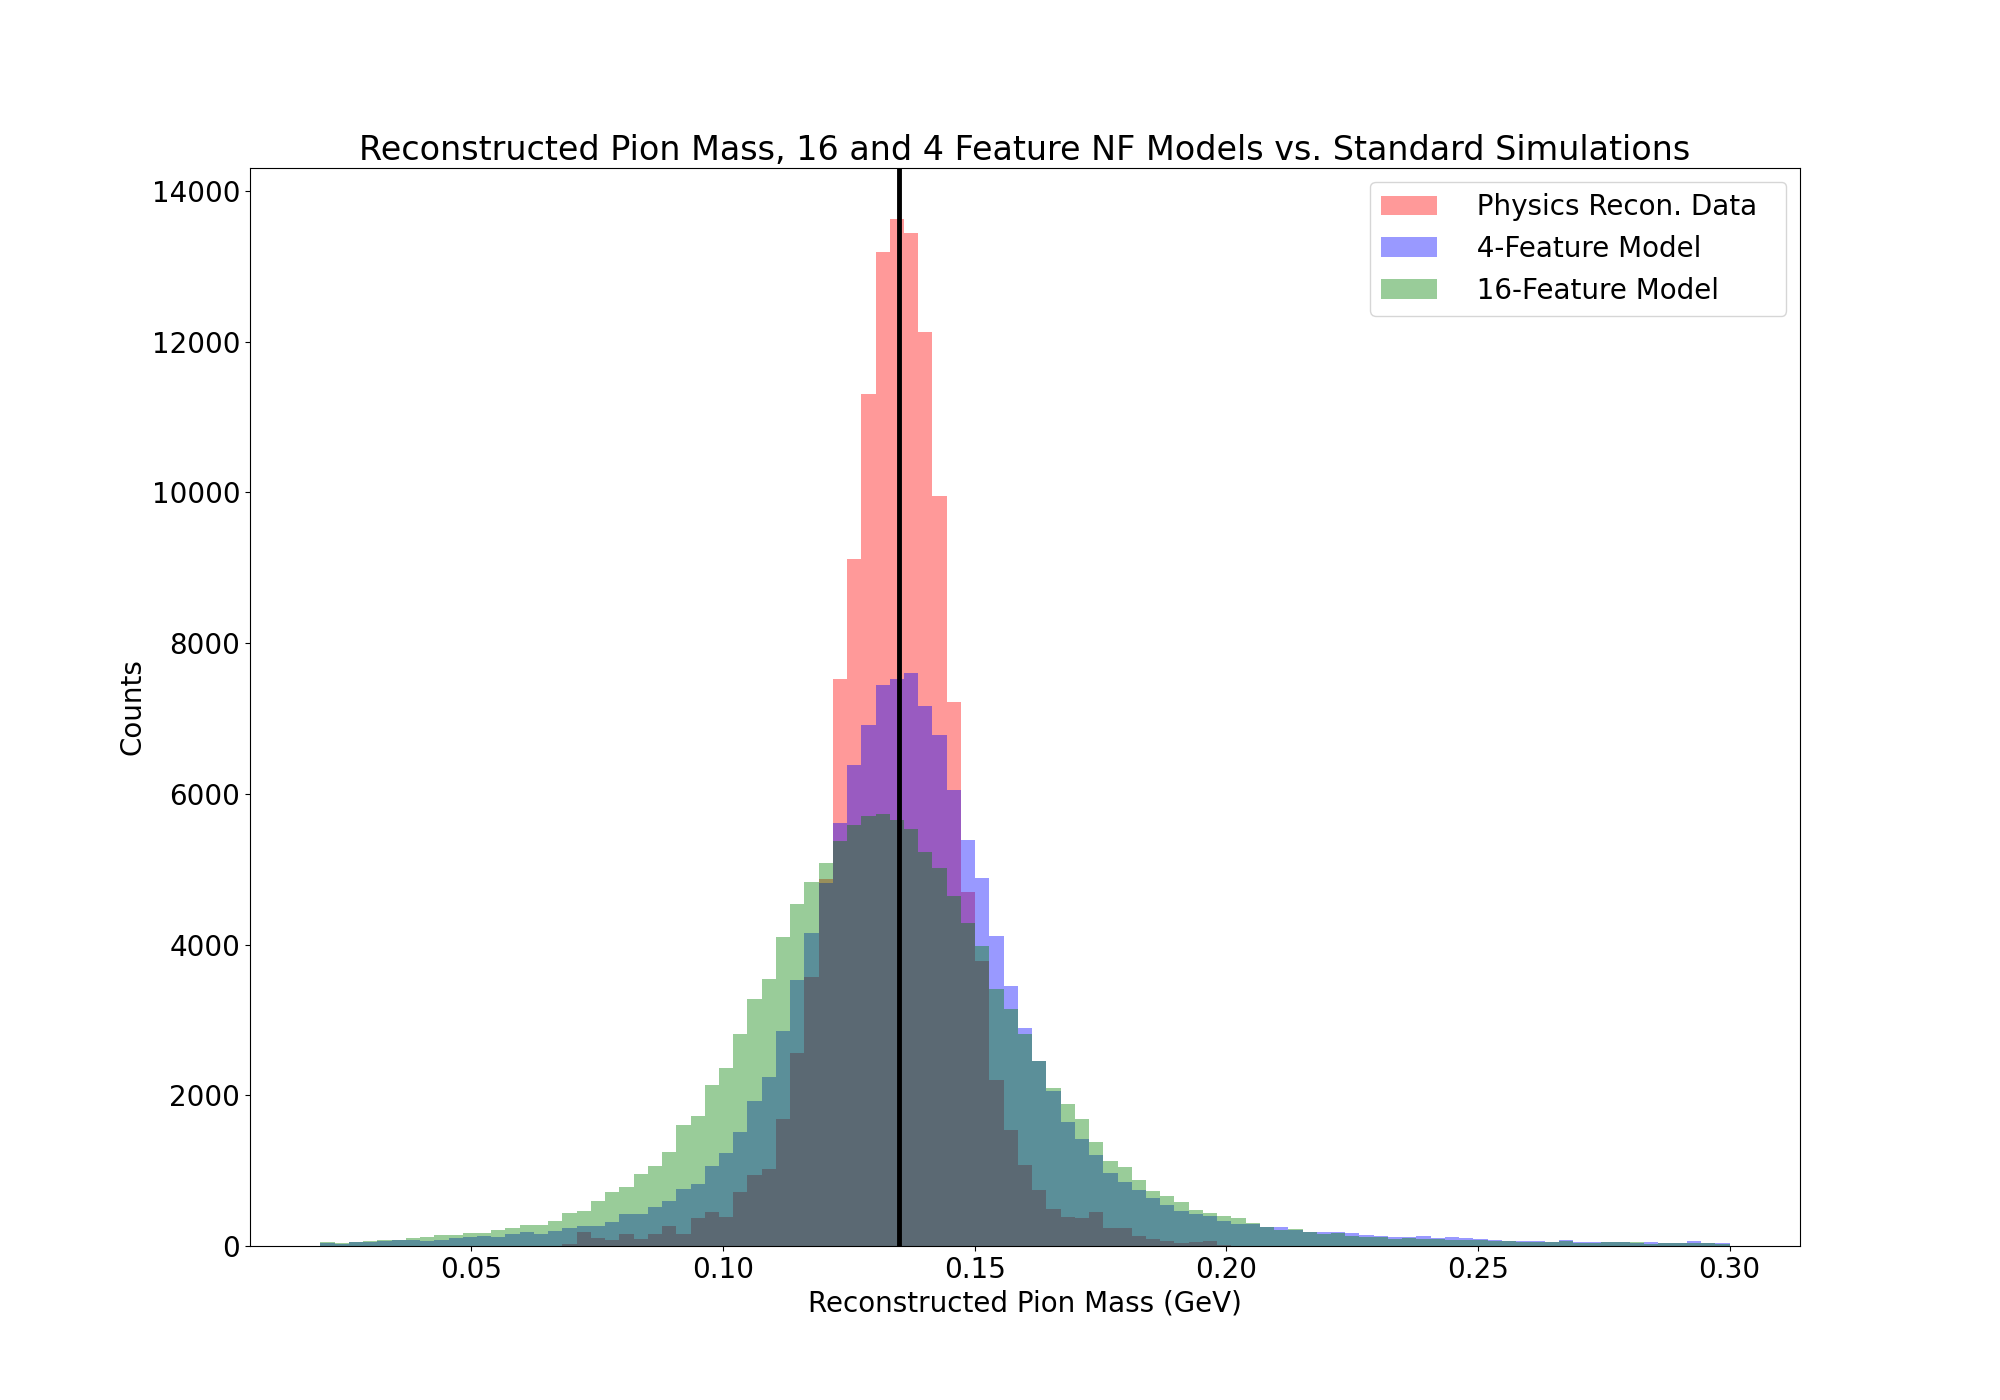
\includegraphics[width = 0.45\textwidth]{Chapters/Ch3-Simulations/normalizing_flows/pics/MeetingFigures/Bobby/Reconstructed_Pion_Mass,_16_and_4_Feature_NF_Models_vs_Standard_Simulations.png}
            \label{fig: jul8_pion_comparison5}
            }
            \subfloat[]{
            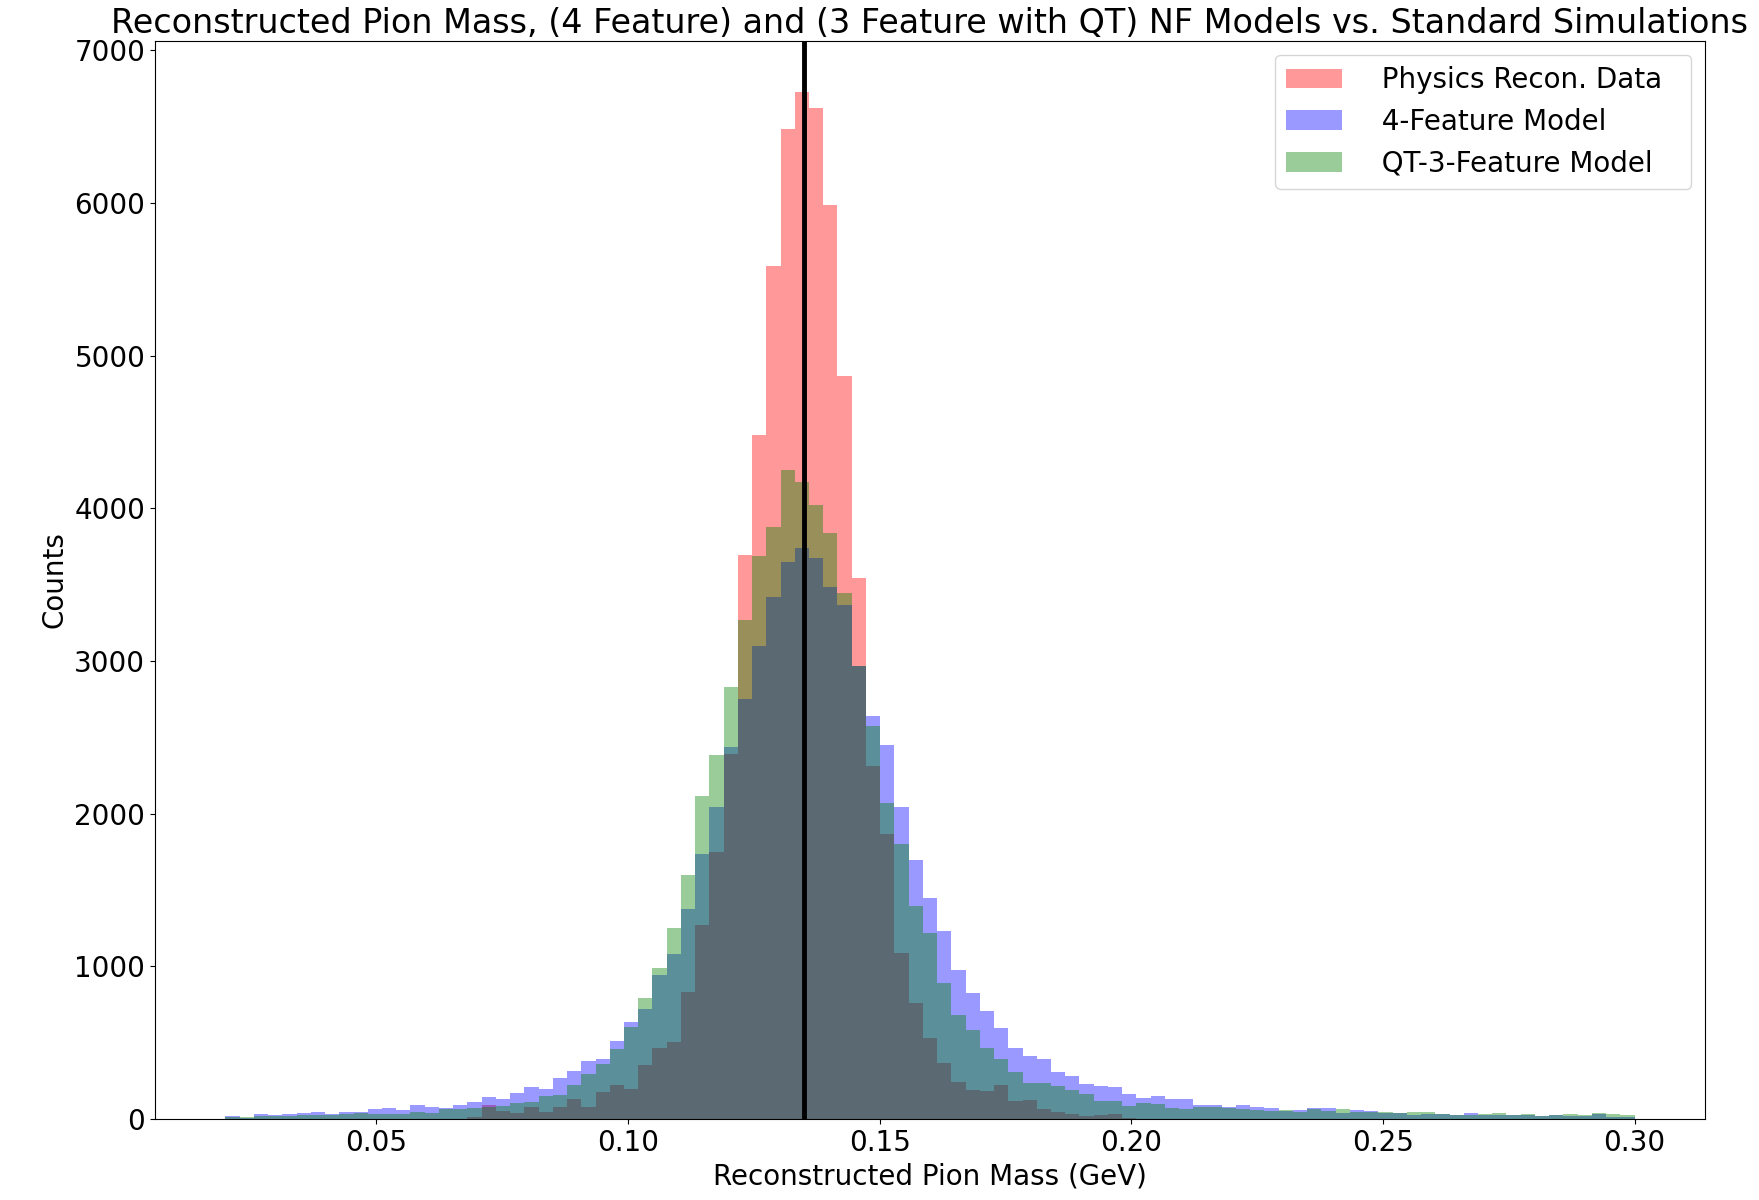
\includegraphics[width = 0.45\textwidth]{Chapters/Ch3-Simulations/normalizing_flows/pics/MeetingFigures/Bobby/qt-3-4.png}
            \label{fig: jul8_pion_comparison}
            }
            \caption[Placeholder Short text]{Comparison of reconstructed pion mass with different training models and preprocessing methods. The left panel shows the approximation of the standard reconstruction pion mass peak using a 4 feature model and a 16 feature model, where the 4 feature model shows a better fit. The right panel demonstrates a slight improvement in the reproduction of the GEANT4 simulated pion peak when preprocessing the feature set with a quantile transformer before training the normalizing flow.}
            \label{fig:combined_pion_comparison}
        \end{figure}


\subsection{Inverse Problems}

    The conditional normalizing flow takes the base distribution $Y$ and the context $Z$ to learn $X$. How do training and sampling work? Ideally, Fig.~\ref{fig: jul8_NF}'s vertical axis should be just 0. 

    
    \begin{figure}[H]
        \centering
        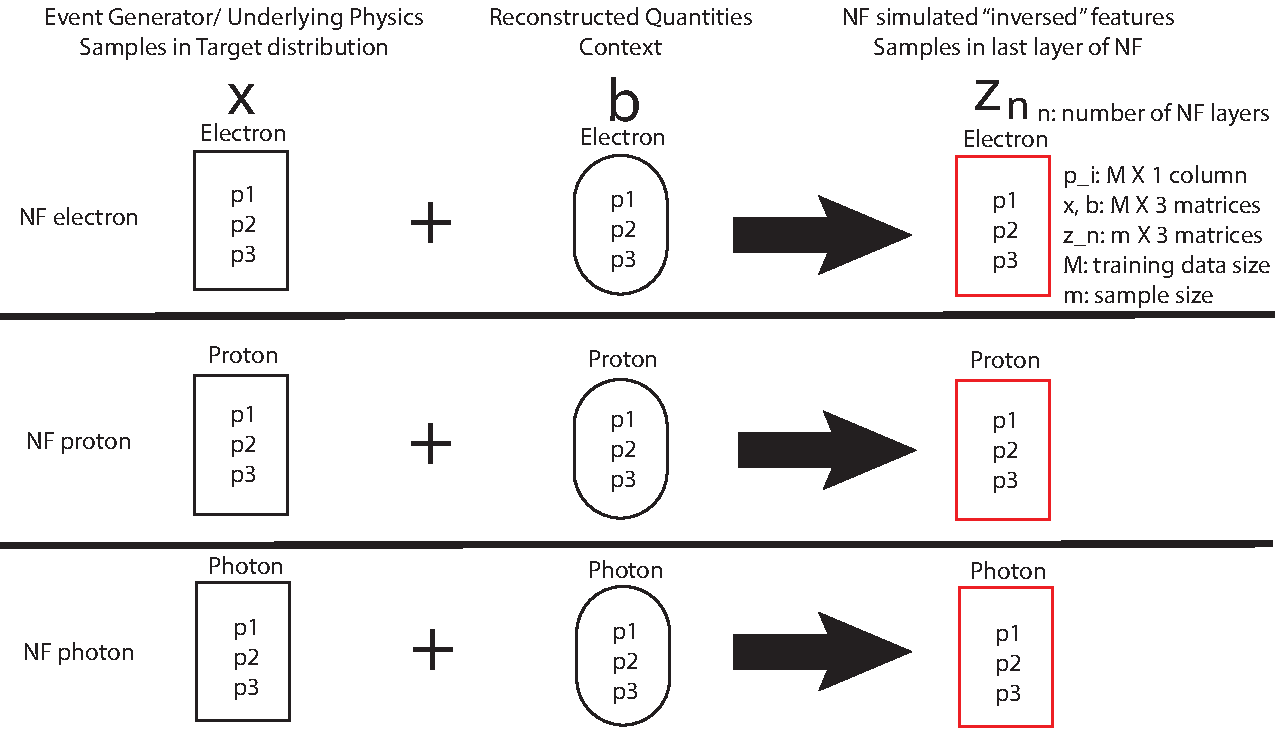
\includegraphics[width=0.8\textwidth]{Chapters/Ch3-Simulations/normalizing_flows/pics/MeetingFigures/Sangbaek/NFdiag1.pdf}
        \caption[Placeholder Short text]{Simplified schematic diagrams to depict the purpose of this project. The NF simulated features should be `similar' to that of underlying physics.}
        \label{fig:goal}
    \end{figure}
    \begin{figure}[H]
        \centering
        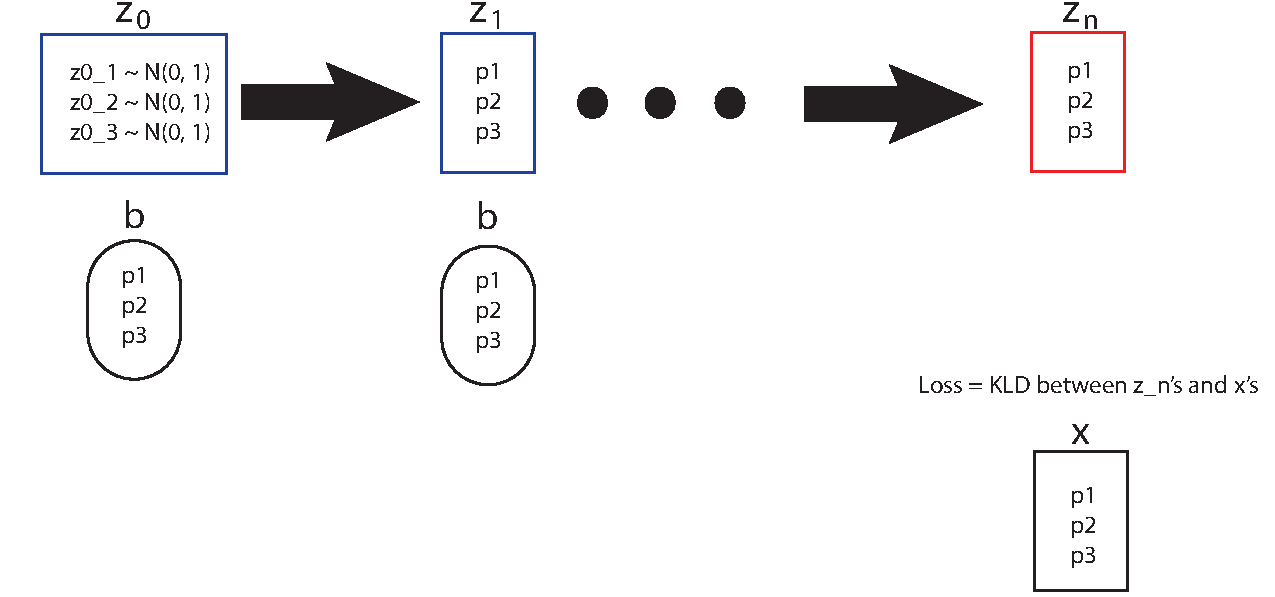
\includegraphics[width=0.8\textwidth]{Chapters/Ch3-Simulations/normalizing_flows/pics/MeetingFigures/Sangbaek/NFdiag2.pdf}
        \caption[Placeholder Short text]{We use the conditional normalizing to realize Fig.~\ref{fig:goal}. We use the experimentally given features (reconstructed features) as context variables. The base distributions, which is the constant distributions, should be transformed to the final layer, $z_2$. The training step repeats the backward propagation to lower the KLD between \{$z_n$\} and \{$x$\}, the features in underlying physics. Please note that we know $x$ only for the simulational data. For this work, I used $n$=2 to make things simple.}
        \label{fig:architecture}
    \end{figure}
    
    Better diagrams are in Figs.~\ref{fig:goal}, \ref{fig:architecture}. As for the benchmark to determine how useful this procedure is, I introduce ``exclusivity" variables for the ``exclusive" reactions. In this fixed target experiment, we know the energies and momenta of particles before the reaction. We measure the momenta of particles after the reaction.
    
    
    
    
    
    \begin{figure}[H]
        \centering
        \begin{minipage}{.5\textwidth}
        
            \centering
           % Electron
            
            %\caption[Placeholder Short text]{(a)}
            \includegraphics[width=.99\textwidth,trim={0 0 0 0},clip]{Chapters/Ch3-Simulations/normalizing_flows/pics/MeetingFigures/Bobby/inverse/gen_Px_1_vs_gen_-_recon_Px_1.png}
            \includegraphics[width=.99\textwidth,trim={0 0 0 0},clip]{Chapters/Ch3-Simulations/normalizing_flows/pics/MeetingFigures/Bobby/inverse/gen_Px_1_vs_gen_-_nf_Px_1.png}
    
            %\caption[Placeholder Short text]{(c)}
        \end{minipage}%
        \begin{minipage}{.5\textwidth}
        
            \centering
           % Electron
            
            %\caption[Placeholder Short text]{(a)}
            \includegraphics[width=.99\textwidth,trim={0 0 0 0},clip]{Chapters/Ch3-Simulations/normalizing_flows/pics/MeetingFigures/Bobby/inverse/gen_Py_1_vs_gen_-_recon_Py_1.png}
            \includegraphics[width=.99\textwidth,trim={0 0 0 0},clip]{Chapters/Ch3-Simulations/normalizing_flows/pics/MeetingFigures/Bobby/inverse/gen_Py_1_vs_gen_-_nf_Py_1.png}
    
            %\caption[Placeholder Short text]{(c)}
        \end{minipage}%
        \caption[Placeholder Short text]{\textbf{TOP:} Truth Event - Reconstructed Event. If standard physics reconstruction algorithms were perfect, we would have a horizontal line at 0 across the distribution (no difference between the reconstructed feature value, and the true feature value, for any event in the data set). \textbf{BOTTOM:} Truth Event - NF estimate of truth event conditional on Reconstructed event values. For the NF to be useful, we would need the difference between the truth event values and the NF estimates to be closer to zero than the differences between just the truth and reconstructed values. However, instead we observe that the spread is about a factor of 2 \textbf{worse} using the NF than not using it at all. }
        \label{fig:16features6}
    \end{figure}
    
    
    I have tried to train the NF to reproduce $x-b$, not $x$ itself because, the 1D distributions of $x-b$'s are more symmetric. This practice clarifies the problem that we have encountered.
    
    Let's focus on only one feature, electron's $p_x$ for example. This time, I used 6 layers of intermediate flows. Fig.~\ref{fig:electron_px} shows that the issue in this probabilistic inverse problem.
    The NF is trained to learn $x-b$ distributions, and it did its job by producing $\mathbf{z_6}-\mathbf{b}$ that follows $\mathbf{x}-\mathbf{b}$. Now, we want $\mathbf{z_6}-\mathbf{b}$ to be exactly 0, but in reality we're seeing a larger variance in the sample $\mathbf{z_6}-\mathbf{x}$.
    
    So, this is my guess about what is happening. Let's oversimplify about the difference. For the single elements,
    \begin{align}
        x -b =& ~a = \pm 1\\
        z_6-b =& ~b = \pm 1\\
        z_6 -x =& (z_6-b) - (x-b) = a- b \neq 0
    \end{align}
    We can only make $a$ and $b$ follow the same distribution, i.e., binary distribution, but $a$ and $b$ are mostly independent without a correct guessing of probability on the sign. So, $a-b$'s distributions are actually convolution of two binary distributions, not 0. So this implies that the conditional NF works really well in terms of reproducing collective behavior, but not in the event by event basis that is required for this study. Actually, there is no feature that is directly related to the signs of $x-b$.
    
    
    
    inverse is an ongoing study
    
    We demonstrate a proof of principle for using a normalizing flow to learn a physics process's probability distribution in order to decrease physics simulation computing time and requirements. In this work, we used traditional physics simulations to generate a dataset $\mathbf{x}$ of 5 million data points with each data point having 16 or 4 features.  We take as input a constant 16D or 4D normal distribution $p(\mathbf{z})$, and examine whether the flow model can learn the transformation to $p(\mathbf{x})$ using a random subset of $\mathbf{x}$ for training. We observed a reasonable agreement between the results of the flow-based modeling and traditional physics methods while achieving a computational speedup factor of 10 to 1,000, but the flow is currently unable to reproduce some fine-detailed structures of the physics process.
    
    
    \parencite{Radhakrishnan2020OverparameterizedMemory}